% Options for packages loaded elsewhere
% Options for packages loaded elsewhere
\PassOptionsToPackage{unicode}{hyperref}
\PassOptionsToPackage{hyphens}{url}
\PassOptionsToPackage{dvipsnames,svgnames,x11names}{xcolor}
%
\documentclass[
  letterpaper,
  DIV=11,
  numbers=noendperiod]{scrartcl}
\usepackage{xcolor}
\usepackage{amsmath,amssymb}
\setcounter{secnumdepth}{-\maxdimen} % remove section numbering
\usepackage{iftex}
\ifPDFTeX
  \usepackage[T1]{fontenc}
  \usepackage[utf8]{inputenc}
  \usepackage{textcomp} % provide euro and other symbols
\else % if luatex or xetex
  \usepackage{unicode-math} % this also loads fontspec
  \defaultfontfeatures{Scale=MatchLowercase}
  \defaultfontfeatures[\rmfamily]{Ligatures=TeX,Scale=1}
\fi
\usepackage{lmodern}
\ifPDFTeX\else
  % xetex/luatex font selection
\fi
% Use upquote if available, for straight quotes in verbatim environments
\IfFileExists{upquote.sty}{\usepackage{upquote}}{}
\IfFileExists{microtype.sty}{% use microtype if available
  \usepackage[]{microtype}
  \UseMicrotypeSet[protrusion]{basicmath} % disable protrusion for tt fonts
}{}
\makeatletter
\@ifundefined{KOMAClassName}{% if non-KOMA class
  \IfFileExists{parskip.sty}{%
    \usepackage{parskip}
  }{% else
    \setlength{\parindent}{0pt}
    \setlength{\parskip}{6pt plus 2pt minus 1pt}}
}{% if KOMA class
  \KOMAoptions{parskip=half}}
\makeatother
% Make \paragraph and \subparagraph free-standing
\makeatletter
\ifx\paragraph\undefined\else
  \let\oldparagraph\paragraph
  \renewcommand{\paragraph}{
    \@ifstar
      \xxxParagraphStar
      \xxxParagraphNoStar
  }
  \newcommand{\xxxParagraphStar}[1]{\oldparagraph*{#1}\mbox{}}
  \newcommand{\xxxParagraphNoStar}[1]{\oldparagraph{#1}\mbox{}}
\fi
\ifx\subparagraph\undefined\else
  \let\oldsubparagraph\subparagraph
  \renewcommand{\subparagraph}{
    \@ifstar
      \xxxSubParagraphStar
      \xxxSubParagraphNoStar
  }
  \newcommand{\xxxSubParagraphStar}[1]{\oldsubparagraph*{#1}\mbox{}}
  \newcommand{\xxxSubParagraphNoStar}[1]{\oldsubparagraph{#1}\mbox{}}
\fi
\makeatother

\usepackage{color}
\usepackage{fancyvrb}
\newcommand{\VerbBar}{|}
\newcommand{\VERB}{\Verb[commandchars=\\\{\}]}
\DefineVerbatimEnvironment{Highlighting}{Verbatim}{commandchars=\\\{\}}
% Add ',fontsize=\small' for more characters per line
\usepackage{framed}
\definecolor{shadecolor}{RGB}{241,243,245}
\newenvironment{Shaded}{\begin{snugshade}}{\end{snugshade}}
\newcommand{\AlertTok}[1]{\textcolor[rgb]{0.68,0.00,0.00}{#1}}
\newcommand{\AnnotationTok}[1]{\textcolor[rgb]{0.37,0.37,0.37}{#1}}
\newcommand{\AttributeTok}[1]{\textcolor[rgb]{0.40,0.45,0.13}{#1}}
\newcommand{\BaseNTok}[1]{\textcolor[rgb]{0.68,0.00,0.00}{#1}}
\newcommand{\BuiltInTok}[1]{\textcolor[rgb]{0.00,0.23,0.31}{#1}}
\newcommand{\CharTok}[1]{\textcolor[rgb]{0.13,0.47,0.30}{#1}}
\newcommand{\CommentTok}[1]{\textcolor[rgb]{0.37,0.37,0.37}{#1}}
\newcommand{\CommentVarTok}[1]{\textcolor[rgb]{0.37,0.37,0.37}{\textit{#1}}}
\newcommand{\ConstantTok}[1]{\textcolor[rgb]{0.56,0.35,0.01}{#1}}
\newcommand{\ControlFlowTok}[1]{\textcolor[rgb]{0.00,0.23,0.31}{\textbf{#1}}}
\newcommand{\DataTypeTok}[1]{\textcolor[rgb]{0.68,0.00,0.00}{#1}}
\newcommand{\DecValTok}[1]{\textcolor[rgb]{0.68,0.00,0.00}{#1}}
\newcommand{\DocumentationTok}[1]{\textcolor[rgb]{0.37,0.37,0.37}{\textit{#1}}}
\newcommand{\ErrorTok}[1]{\textcolor[rgb]{0.68,0.00,0.00}{#1}}
\newcommand{\ExtensionTok}[1]{\textcolor[rgb]{0.00,0.23,0.31}{#1}}
\newcommand{\FloatTok}[1]{\textcolor[rgb]{0.68,0.00,0.00}{#1}}
\newcommand{\FunctionTok}[1]{\textcolor[rgb]{0.28,0.35,0.67}{#1}}
\newcommand{\ImportTok}[1]{\textcolor[rgb]{0.00,0.46,0.62}{#1}}
\newcommand{\InformationTok}[1]{\textcolor[rgb]{0.37,0.37,0.37}{#1}}
\newcommand{\KeywordTok}[1]{\textcolor[rgb]{0.00,0.23,0.31}{\textbf{#1}}}
\newcommand{\NormalTok}[1]{\textcolor[rgb]{0.00,0.23,0.31}{#1}}
\newcommand{\OperatorTok}[1]{\textcolor[rgb]{0.37,0.37,0.37}{#1}}
\newcommand{\OtherTok}[1]{\textcolor[rgb]{0.00,0.23,0.31}{#1}}
\newcommand{\PreprocessorTok}[1]{\textcolor[rgb]{0.68,0.00,0.00}{#1}}
\newcommand{\RegionMarkerTok}[1]{\textcolor[rgb]{0.00,0.23,0.31}{#1}}
\newcommand{\SpecialCharTok}[1]{\textcolor[rgb]{0.37,0.37,0.37}{#1}}
\newcommand{\SpecialStringTok}[1]{\textcolor[rgb]{0.13,0.47,0.30}{#1}}
\newcommand{\StringTok}[1]{\textcolor[rgb]{0.13,0.47,0.30}{#1}}
\newcommand{\VariableTok}[1]{\textcolor[rgb]{0.07,0.07,0.07}{#1}}
\newcommand{\VerbatimStringTok}[1]{\textcolor[rgb]{0.13,0.47,0.30}{#1}}
\newcommand{\WarningTok}[1]{\textcolor[rgb]{0.37,0.37,0.37}{\textit{#1}}}

\usepackage{longtable,booktabs,array}
\usepackage{calc} % for calculating minipage widths
% Correct order of tables after \paragraph or \subparagraph
\usepackage{etoolbox}
\makeatletter
\patchcmd\longtable{\par}{\if@noskipsec\mbox{}\fi\par}{}{}
\makeatother
% Allow footnotes in longtable head/foot
\IfFileExists{footnotehyper.sty}{\usepackage{footnotehyper}}{\usepackage{footnote}}
\makesavenoteenv{longtable}
\usepackage{graphicx}
\makeatletter
\newsavebox\pandoc@box
\newcommand*\pandocbounded[1]{% scales image to fit in text height/width
  \sbox\pandoc@box{#1}%
  \Gscale@div\@tempa{\textheight}{\dimexpr\ht\pandoc@box+\dp\pandoc@box\relax}%
  \Gscale@div\@tempb{\linewidth}{\wd\pandoc@box}%
  \ifdim\@tempb\p@<\@tempa\p@\let\@tempa\@tempb\fi% select the smaller of both
  \ifdim\@tempa\p@<\p@\scalebox{\@tempa}{\usebox\pandoc@box}%
  \else\usebox{\pandoc@box}%
  \fi%
}
% Set default figure placement to htbp
\def\fps@figure{htbp}
\makeatother





\setlength{\emergencystretch}{3em} % prevent overfull lines

\providecommand{\tightlist}{%
  \setlength{\itemsep}{0pt}\setlength{\parskip}{0pt}}



 


\KOMAoption{captions}{tableheading}
\makeatletter
\@ifpackageloaded{caption}{}{\usepackage{caption}}
\AtBeginDocument{%
\ifdefined\contentsname
  \renewcommand*\contentsname{Table of contents}
\else
  \newcommand\contentsname{Table of contents}
\fi
\ifdefined\listfigurename
  \renewcommand*\listfigurename{List of Figures}
\else
  \newcommand\listfigurename{List of Figures}
\fi
\ifdefined\listtablename
  \renewcommand*\listtablename{List of Tables}
\else
  \newcommand\listtablename{List of Tables}
\fi
\ifdefined\figurename
  \renewcommand*\figurename{Figure}
\else
  \newcommand\figurename{Figure}
\fi
\ifdefined\tablename
  \renewcommand*\tablename{Table}
\else
  \newcommand\tablename{Table}
\fi
}
\@ifpackageloaded{float}{}{\usepackage{float}}
\floatstyle{ruled}
\@ifundefined{c@chapter}{\newfloat{codelisting}{h}{lop}}{\newfloat{codelisting}{h}{lop}[chapter]}
\floatname{codelisting}{Listing}
\newcommand*\listoflistings{\listof{codelisting}{List of Listings}}
\makeatother
\makeatletter
\makeatother
\makeatletter
\@ifpackageloaded{caption}{}{\usepackage{caption}}
\@ifpackageloaded{subcaption}{}{\usepackage{subcaption}}
\makeatother
\usepackage{bookmark}
\IfFileExists{xurl.sty}{\usepackage{xurl}}{} % add URL line breaks if available
\urlstyle{same}
\hypersetup{
  pdftitle={Cocoa Price Forecasting: Weighted Local Linear vs Machine Learning Methods},
  colorlinks=true,
  linkcolor={blue},
  filecolor={Maroon},
  citecolor={Blue},
  urlcolor={Blue},
  pdfcreator={LaTeX via pandoc}}


\title{Cocoa Price Forecasting: Weighted Local Linear vs Machine
Learning Methods}
\author{}
\date{}
\begin{document}
\maketitle


\textbf{Project:} Empirical Validation of the CGS Weighted Local Linear
Framework

\textbf{Reference:} CGS (2025) - Nonparametric Time Series Forecasting
with Structural Breaks

\begin{center}\rule{0.5\linewidth}{0.5pt}\end{center}

\subsection{Abstract}\label{abstract}

This notebook implements the experimental framework to validate the CGS
weighted local linear methodology on cocoa price data.

\subsubsection{Models Evaluated}\label{models-evaluated}

\begin{longtable}[]{@{}
  >{\raggedright\arraybackslash}p{(\linewidth - 6\tabcolsep) * \real{0.2381}}
  >{\raggedright\arraybackslash}p{(\linewidth - 6\tabcolsep) * \real{0.1667}}
  >{\raggedright\arraybackslash}p{(\linewidth - 6\tabcolsep) * \real{0.2857}}
  >{\raggedright\arraybackslash}p{(\linewidth - 6\tabcolsep) * \real{0.3095}}@{}}
\toprule\noalign{}
\begin{minipage}[b]{\linewidth}\raggedright
Category
\end{minipage} & \begin{minipage}[b]{\linewidth}\raggedright
Model
\end{minipage} & \begin{minipage}[b]{\linewidth}\raggedright
Data Usage
\end{minipage} & \begin{minipage}[b]{\linewidth}\raggedright
Description
\end{minipage} \\
\midrule\noalign{}
\endhead
\bottomrule\noalign{}
\endlastfoot
NP Benchmarks & Pre-Break LL & Pre-break only & High bias, low variance
baseline \\
& Post-Break LL & Post-break only & Low bias, high variance baseline \\
& Weighted LL (WLL) & Combined & CGS convex combination with MFV-tuned
gamma \\
ML Competitors & Random Forest & Full sample & Ensemble bagging
method \\
& XGBoost & Full sample & Gradient boosting method \\
ML Extension & RF Weighted Combo & Combined & CGS weighting applied to
RF \\
& XGB Weighted Combo & Combined & CGS weighting applied to XGB \\
\end{longtable}

\subsubsection{Evaluation Metrics}\label{evaluation-metrics}

\begin{itemize}
\tightlist
\item
  \textbf{Primary:} Out-of-Sample Mean Squared Forecast Error (MSFE)
\item
  \textbf{Secondary:} Modified Diebold-Mariano (MDM) test for pairwise
  comparisons
\end{itemize}

\subsection{1. Environment Setup}\label{environment-setup}

\begin{Shaded}
\begin{Highlighting}[]
\CommentTok{\# Install required packages}
\ImportTok{import}\NormalTok{ subprocess}
\ImportTok{import}\NormalTok{ sys}

\CommentTok{\# Install torch (required for NP models) and the local package}
\NormalTok{subprocess.check\_call([sys.executable, }\StringTok{\textquotesingle{}{-}m\textquotesingle{}}\NormalTok{, }\StringTok{\textquotesingle{}pip\textquotesingle{}}\NormalTok{, }\StringTok{\textquotesingle{}install\textquotesingle{}}\NormalTok{, }\StringTok{\textquotesingle{}torch\textquotesingle{}}\NormalTok{, }\StringTok{\textquotesingle{}{-}q\textquotesingle{}}\NormalTok{])}
\NormalTok{subprocess.check\_call([sys.executable, }\StringTok{\textquotesingle{}{-}m\textquotesingle{}}\NormalTok{, }\StringTok{\textquotesingle{}pip\textquotesingle{}}\NormalTok{, }\StringTok{\textquotesingle{}install\textquotesingle{}}\NormalTok{, }\StringTok{\textquotesingle{}{-}e\textquotesingle{}}\NormalTok{, }\StringTok{\textquotesingle{}..\textquotesingle{}}\NormalTok{, }\StringTok{\textquotesingle{}{-}q\textquotesingle{}}\NormalTok{])}

\BuiltInTok{print}\NormalTok{(}\StringTok{\textquotesingle{}Dependencies installed successfully.\textquotesingle{}}\NormalTok{)}
\end{Highlighting}
\end{Shaded}

\begin{verbatim}
Dependencies installed successfully.
\end{verbatim}

\begin{Shaded}
\begin{Highlighting}[]
\ImportTok{import}\NormalTok{ warnings}
\NormalTok{warnings.filterwarnings(}\StringTok{\textquotesingle{}ignore\textquotesingle{}}\NormalTok{)}

\ImportTok{import}\NormalTok{ numpy }\ImportTok{as}\NormalTok{ np}
\ImportTok{import}\NormalTok{ pandas }\ImportTok{as}\NormalTok{ pd}
\ImportTok{import}\NormalTok{ matplotlib.pyplot }\ImportTok{as}\NormalTok{ plt}
\ImportTok{from}\NormalTok{ pathlib }\ImportTok{import}\NormalTok{ Path}
\ImportTok{from}\NormalTok{ itertools }\ImportTok{import}\NormalTok{ product}
\ImportTok{from}\NormalTok{ typing }\ImportTok{import}\NormalTok{ Dict, Any, List, Tuple}
\ImportTok{from}\NormalTok{ scipy }\ImportTok{import}\NormalTok{ stats}
\ImportTok{from}\NormalTok{ datetime }\ImportTok{import}\NormalTok{ datetime}

\CommentTok{\# Plotting configuration}
\NormalTok{plt.style.use(}\StringTok{\textquotesingle{}seaborn{-}v0\_8{-}whitegrid\textquotesingle{}}\NormalTok{)}
\NormalTok{plt.rcParams[}\StringTok{\textquotesingle{}figure.figsize\textquotesingle{}}\NormalTok{] }\OperatorTok{=}\NormalTok{ (}\DecValTok{12}\NormalTok{, }\DecValTok{6}\NormalTok{)}
\NormalTok{plt.rcParams[}\StringTok{\textquotesingle{}font.size\textquotesingle{}}\NormalTok{] }\OperatorTok{=} \DecValTok{11}

\CommentTok{\# Color scheme for models}
\NormalTok{COLORS }\OperatorTok{=}\NormalTok{ \{}
    \StringTok{\textquotesingle{}pre\_break\textquotesingle{}}\NormalTok{: }\StringTok{\textquotesingle{}\#E74C3C\textquotesingle{}}\NormalTok{,}
    \StringTok{\textquotesingle{}post\_break\textquotesingle{}}\NormalTok{: }\StringTok{\textquotesingle{}\#3498DB\textquotesingle{}}\NormalTok{,}
    \StringTok{\textquotesingle{}wll\textquotesingle{}}\NormalTok{: }\StringTok{\textquotesingle{}\#2ECC71\textquotesingle{}}\NormalTok{,}
    \StringTok{\textquotesingle{}rf\textquotesingle{}}\NormalTok{: }\StringTok{\textquotesingle{}\#9B59B6\textquotesingle{}}\NormalTok{,}
    \StringTok{\textquotesingle{}xgb\textquotesingle{}}\NormalTok{: }\StringTok{\textquotesingle{}\#F39C12\textquotesingle{}}\NormalTok{,}
    \StringTok{\textquotesingle{}rf\_combo\textquotesingle{}}\NormalTok{: }\StringTok{\textquotesingle{}\#1ABC9C\textquotesingle{}}\NormalTok{,}
    \StringTok{\textquotesingle{}xgb\_combo\textquotesingle{}}\NormalTok{: }\StringTok{\textquotesingle{}\#E67E22\textquotesingle{}}\NormalTok{,}
\NormalTok{\}}

\BuiltInTok{print}\NormalTok{(}\StringTok{\textquotesingle{}Standard libraries imported.\textquotesingle{}}\NormalTok{)}
\end{Highlighting}
\end{Shaded}

\begin{verbatim}
Standard libraries imported.
\end{verbatim}

\begin{Shaded}
\begin{Highlighting}[]
\CommentTok{\# Project modules}
\ImportTok{import}\NormalTok{ sys}
\NormalTok{sys.path.insert(}\DecValTok{0}\NormalTok{, }\BuiltInTok{str}\NormalTok{(Path.cwd().parent }\OperatorTok{/} \StringTok{\textquotesingle{}src\textquotesingle{}}\NormalTok{))}

\ImportTok{from}\NormalTok{ cocoa.data.features }\ImportTok{import}\NormalTok{ build\_features}
\ImportTok{from}\NormalTok{ cocoa.models.np\_combo }\ImportTok{import}\NormalTok{ NPConvexCombinationModel}
\ImportTok{from}\NormalTok{ cocoa.models.np\_regime }\ImportTok{import}\NormalTok{ NPRegimeModel}
\ImportTok{from}\NormalTok{ cocoa.models.np\_engines }\ImportTok{import}\NormalTok{ LocalPolynomialEngine}
\ImportTok{from}\NormalTok{ cocoa.models.np\_kernels }\ImportTok{import}\NormalTok{ EpanechnikovKernel}
\ImportTok{from}\NormalTok{ cocoa.models.ml\_models }\ImportTok{import}\NormalTok{ RFModel, XGBModel}
\ImportTok{from}\NormalTok{ cocoa.models.ml\_combo }\ImportTok{import}\NormalTok{ MLConvexCombinationModel}
\ImportTok{from}\NormalTok{ cocoa.models.bandwidth }\ImportTok{import}\NormalTok{ create\_precentered\_grid}
\ImportTok{from}\NormalTok{ cocoa.models.mfv\_CV }\ImportTok{import}\NormalTok{ MFVValidator, MFVConvexComboValidator}
\ImportTok{from}\NormalTok{ cocoa.models.evaluation }\ImportTok{import}\NormalTok{ mean\_squared\_error}
\ImportTok{from}\NormalTok{ cocoa.models.assets }\ImportTok{import}\NormalTok{ (}
\NormalTok{    BREAK\_ID\_ONE\_BASED, OOS\_START\_DATE, PROCESSED\_DATA\_PATH,}
\NormalTok{    DEFAULT\_FEATURE\_COLS, DEFAULT\_TARGET\_COL, Q\_VALUE,}
\NormalTok{    RF\_PARAM\_GRID, XGB\_PARAM\_GRID,}
\NormalTok{)}

\BuiltInTok{print}\NormalTok{(}\StringTok{\textquotesingle{}Project modules imported.\textquotesingle{}}\NormalTok{)}
\end{Highlighting}
\end{Shaded}

\begin{verbatim}
Project modules imported.
\end{verbatim}

\subsection{2. Data Loading and
Exploration}\label{data-loading-and-exploration}

\begin{Shaded}
\begin{Highlighting}[]
\CommentTok{\# Load processed data}
\NormalTok{DATA\_PATH }\OperatorTok{=}\NormalTok{ Path(PROCESSED\_DATA\_PATH)}

\ControlFlowTok{if} \KeywordTok{not}\NormalTok{ DATA\_PATH.exists():}
    \BuiltInTok{print}\NormalTok{(}\StringTok{\textquotesingle{}Processed data not found. Building from raw data...\textquotesingle{}}\NormalTok{)}
\NormalTok{    project\_root }\OperatorTok{=}\NormalTok{ Path.cwd().parent}
\NormalTok{    df }\OperatorTok{=}\NormalTok{ build\_features(}
\NormalTok{        project\_root }\OperatorTok{/} \StringTok{\textquotesingle{}data\textquotesingle{}} \OperatorTok{/} \StringTok{\textquotesingle{}raw\textquotesingle{}}\NormalTok{,}
\NormalTok{        project\_root }\OperatorTok{/} \StringTok{\textquotesingle{}data\textquotesingle{}} \OperatorTok{/} \StringTok{\textquotesingle{}processed\textquotesingle{}}\NormalTok{,}
\NormalTok{        reading\_path}\OperatorTok{=}\StringTok{\textquotesingle{}Ghana\_data\_full.csv\textquotesingle{}}\NormalTok{,}
\NormalTok{        file\_name}\OperatorTok{=}\StringTok{\textquotesingle{}cocoa\_ghana\_full.csv\textquotesingle{}}
\NormalTok{    )}
\ControlFlowTok{else}\NormalTok{:}
\NormalTok{    df }\OperatorTok{=}\NormalTok{ pd.read\_csv(DATA\_PATH)}

\NormalTok{df[}\StringTok{\textquotesingle{}date\textquotesingle{}}\NormalTok{] }\OperatorTok{=}\NormalTok{ pd.to\_datetime(df[}\StringTok{\textquotesingle{}date\textquotesingle{}}\NormalTok{])}
\NormalTok{df }\OperatorTok{=}\NormalTok{ df.sort\_values(}\StringTok{\textquotesingle{}date\textquotesingle{}}\NormalTok{).reset\_index(drop}\OperatorTok{=}\VariableTok{True}\NormalTok{)}

\BuiltInTok{print}\NormalTok{(}\SpecialStringTok{f\textquotesingle{}Dataset: }\SpecialCharTok{\{}\BuiltInTok{len}\NormalTok{(df)}\SpecialCharTok{:,\}}\SpecialStringTok{ observations\textquotesingle{}}\NormalTok{)}
\BuiltInTok{print}\NormalTok{(}\SpecialStringTok{f\textquotesingle{}Date range: }\SpecialCharTok{\{}\NormalTok{df[}\StringTok{"date"}\NormalTok{]}\SpecialCharTok{.}\BuiltInTok{min}\NormalTok{()}\SpecialCharTok{.}\NormalTok{strftime(}\StringTok{"\%Y{-}\%m{-}}\SpecialCharTok{\%d}\StringTok{"}\NormalTok{)}\SpecialCharTok{\}}\SpecialStringTok{ to }\SpecialCharTok{\{}\NormalTok{df[}\StringTok{"date"}\NormalTok{]}\SpecialCharTok{.}\BuiltInTok{max}\NormalTok{()}\SpecialCharTok{.}\NormalTok{strftime(}\StringTok{"\%Y{-}\%m{-}}\SpecialCharTok{\%d}\StringTok{"}\NormalTok{)}\SpecialCharTok{\}}\SpecialStringTok{\textquotesingle{}}\NormalTok{)}
\BuiltInTok{print}\NormalTok{(}\SpecialStringTok{f\textquotesingle{}Columns: }\SpecialCharTok{\{}\BuiltInTok{list}\NormalTok{(df.columns)}\SpecialCharTok{\}}\SpecialStringTok{\textquotesingle{}}\NormalTok{)}
\NormalTok{df.head()}
\end{Highlighting}
\end{Shaded}

\begin{verbatim}
Dataset: 6,734 observations
Date range: 1994-10-04 to 2025-02-26
Columns: ['date', 'PRCP_anom_mean', 'TAVG_anom_mean', 'PRCP_anom_std', 'TAVG_anom_std', 'N_stations', 'log_price', 'log_price_lagt', 'log_return', 'log_return_forecast_target']
\end{verbatim}

\begin{longtable}[]{@{}lllllllllll@{}}
\toprule\noalign{}
& date & PRCP\_anom\_mean & TAVG\_anom\_mean & PRCP\_anom\_std &
TAVG\_anom\_std & N\_stations & log\_price & log\_price\_lagt &
log\_return & log\_return\_forecast\_target \\
\midrule\noalign{}
\endhead
\bottomrule\noalign{}
\endlastfoot
0 & 1994-10-04 & 0.0000 & 0.25 & 0.000000 & 0.000000 & 1 & 7.287752 &
7.290457 & -0.002704 & -0.021924 \\
1 & 1994-10-05 & 0.0925 & 0.00 & 0.137886 & 2.828427 & 2 & 7.265828 &
7.287752 & -0.021924 & -0.000175 \\
2 & 1994-10-06 & 0.0040 & -0.40 & 0.005657 & 0.565685 & 2 & 7.265653 &
7.265828 & -0.000175 & -0.009737 \\
3 & 1994-10-07 & -0.0284 & 0.46 & 0.377151 & 1.306905 & 5 & 7.255916 &
7.265653 & -0.009737 & -0.001929 \\
4 & 1994-10-10 & -0.4325 & -4.00 & 0.000000 & 0.000000 & 1 & 7.253987 &
7.255916 & -0.001929 & 0.000149 \\
\end{longtable}

\begin{Shaded}
\begin{Highlighting}[]
\CommentTok{\# Structural break configuration}
\NormalTok{BREAK\_INDEX }\OperatorTok{=}\NormalTok{ BREAK\_ID\_ONE\_BASED }\OperatorTok{{-}} \DecValTok{1}  \CommentTok{\# Convert to 0{-}based}
\NormalTok{BREAK\_DATE }\OperatorTok{=}\NormalTok{ df.iloc[BREAK\_INDEX][}\StringTok{\textquotesingle{}date\textquotesingle{}}\NormalTok{]}

\BuiltInTok{print}\NormalTok{(}\SpecialStringTok{f\textquotesingle{}Structural Break Configuration:\textquotesingle{}}\NormalTok{)}
\BuiltInTok{print}\NormalTok{(}\SpecialStringTok{f\textquotesingle{}  Break Index: }\SpecialCharTok{\{}\NormalTok{BREAK\_INDEX}\SpecialCharTok{\}}\SpecialStringTok{\textquotesingle{}}\NormalTok{)}
\BuiltInTok{print}\NormalTok{(}\SpecialStringTok{f\textquotesingle{}  Break Date: }\SpecialCharTok{\{}\NormalTok{BREAK\_DATE}\SpecialCharTok{.}\NormalTok{strftime(}\StringTok{"\%Y{-}\%m{-}}\SpecialCharTok{\%d}\StringTok{"}\NormalTok{)}\SpecialCharTok{\}}\SpecialStringTok{\textquotesingle{}}\NormalTok{)}
\BuiltInTok{print}\NormalTok{(}\SpecialStringTok{f\textquotesingle{}  Pre{-}break observations: }\SpecialCharTok{\{}\NormalTok{BREAK\_INDEX}\SpecialCharTok{:,\}}\SpecialStringTok{\textquotesingle{}}\NormalTok{)}
\BuiltInTok{print}\NormalTok{(}\SpecialStringTok{f\textquotesingle{}  Post{-}break observations: }\SpecialCharTok{\{}\BuiltInTok{len}\NormalTok{(df) }\OperatorTok{{-}}\NormalTok{ BREAK\_INDEX}\SpecialCharTok{:,\}}\SpecialStringTok{\textquotesingle{}}\NormalTok{)}

\CommentTok{\# Visualization}
\NormalTok{fig, axes }\OperatorTok{=}\NormalTok{ plt.subplots(}\DecValTok{2}\NormalTok{, }\DecValTok{1}\NormalTok{, figsize}\OperatorTok{=}\NormalTok{(}\DecValTok{14}\NormalTok{, }\DecValTok{10}\NormalTok{))}

\CommentTok{\# Log Price}
\NormalTok{ax1 }\OperatorTok{=}\NormalTok{ axes[}\DecValTok{0}\NormalTok{]}
\NormalTok{ax1.plot(df[}\StringTok{\textquotesingle{}date\textquotesingle{}}\NormalTok{], df[}\StringTok{\textquotesingle{}log\_price\textquotesingle{}}\NormalTok{], color}\OperatorTok{=}\StringTok{\textquotesingle{}\#2C3E50\textquotesingle{}}\NormalTok{, linewidth}\OperatorTok{=}\FloatTok{0.8}\NormalTok{)}
\NormalTok{ax1.axvline(x}\OperatorTok{=}\NormalTok{BREAK\_DATE, color}\OperatorTok{=}\StringTok{\textquotesingle{}\#E74C3C\textquotesingle{}}\NormalTok{, linestyle}\OperatorTok{=}\StringTok{\textquotesingle{}{-}{-}\textquotesingle{}}\NormalTok{, linewidth}\OperatorTok{=}\DecValTok{2}\NormalTok{,}
\NormalTok{            label}\OperatorTok{=}\SpecialStringTok{f\textquotesingle{}Structural Break (}\SpecialCharTok{\{}\NormalTok{BREAK\_DATE}\SpecialCharTok{.}\NormalTok{strftime(}\StringTok{"\%Y{-}\%m{-}}\SpecialCharTok{\%d}\StringTok{"}\NormalTok{)}\SpecialCharTok{\}}\SpecialStringTok{)\textquotesingle{}}\NormalTok{)}
\NormalTok{ax1.fill\_between(df[}\StringTok{\textquotesingle{}date\textquotesingle{}}\NormalTok{], df[}\StringTok{\textquotesingle{}log\_price\textquotesingle{}}\NormalTok{].}\BuiltInTok{min}\NormalTok{(), df[}\StringTok{\textquotesingle{}log\_price\textquotesingle{}}\NormalTok{].}\BuiltInTok{max}\NormalTok{(),}
\NormalTok{                 where}\OperatorTok{=}\NormalTok{df[}\StringTok{\textquotesingle{}date\textquotesingle{}}\NormalTok{] }\OperatorTok{\textless{}}\NormalTok{ BREAK\_DATE, alpha}\OperatorTok{=}\FloatTok{0.1}\NormalTok{, color}\OperatorTok{=}\NormalTok{COLORS[}\StringTok{\textquotesingle{}pre\_break\textquotesingle{}}\NormalTok{])}
\NormalTok{ax1.fill\_between(df[}\StringTok{\textquotesingle{}date\textquotesingle{}}\NormalTok{], df[}\StringTok{\textquotesingle{}log\_price\textquotesingle{}}\NormalTok{].}\BuiltInTok{min}\NormalTok{(), df[}\StringTok{\textquotesingle{}log\_price\textquotesingle{}}\NormalTok{].}\BuiltInTok{max}\NormalTok{(),}
\NormalTok{                 where}\OperatorTok{=}\NormalTok{df[}\StringTok{\textquotesingle{}date\textquotesingle{}}\NormalTok{] }\OperatorTok{\textgreater{}=}\NormalTok{ BREAK\_DATE, alpha}\OperatorTok{=}\FloatTok{0.1}\NormalTok{, color}\OperatorTok{=}\NormalTok{COLORS[}\StringTok{\textquotesingle{}post\_break\textquotesingle{}}\NormalTok{])}
\NormalTok{ax1.set\_ylabel(}\StringTok{\textquotesingle{}Log Price\textquotesingle{}}\NormalTok{)}
\NormalTok{ax1.set\_title(}\StringTok{\textquotesingle{}Cocoa Log Price with Structural Break\textquotesingle{}}\NormalTok{)}
\NormalTok{ax1.legend(loc}\OperatorTok{=}\StringTok{\textquotesingle{}upper left\textquotesingle{}}\NormalTok{)}
\NormalTok{ax1.grid(}\VariableTok{True}\NormalTok{, alpha}\OperatorTok{=}\FloatTok{0.3}\NormalTok{)}

\CommentTok{\# Log Returns}
\NormalTok{ax2 }\OperatorTok{=}\NormalTok{ axes[}\DecValTok{1}\NormalTok{]}
\NormalTok{ax2.plot(df[}\StringTok{\textquotesingle{}date\textquotesingle{}}\NormalTok{], df[}\StringTok{\textquotesingle{}log\_return\textquotesingle{}}\NormalTok{], color}\OperatorTok{=}\StringTok{\textquotesingle{}\#2C3E50\textquotesingle{}}\NormalTok{, linewidth}\OperatorTok{=}\FloatTok{0.5}\NormalTok{, alpha}\OperatorTok{=}\FloatTok{0.7}\NormalTok{)}
\NormalTok{ax2.axvline(x}\OperatorTok{=}\NormalTok{BREAK\_DATE, color}\OperatorTok{=}\StringTok{\textquotesingle{}\#E74C3C\textquotesingle{}}\NormalTok{, linestyle}\OperatorTok{=}\StringTok{\textquotesingle{}{-}{-}\textquotesingle{}}\NormalTok{, linewidth}\OperatorTok{=}\DecValTok{2}\NormalTok{)}
\NormalTok{ax2.axhline(y}\OperatorTok{=}\DecValTok{0}\NormalTok{, color}\OperatorTok{=}\StringTok{\textquotesingle{}gray\textquotesingle{}}\NormalTok{, linestyle}\OperatorTok{=}\StringTok{\textquotesingle{}{-}\textquotesingle{}}\NormalTok{, linewidth}\OperatorTok{=}\FloatTok{0.5}\NormalTok{)}
\NormalTok{ax2.set\_xlabel(}\StringTok{\textquotesingle{}Date\textquotesingle{}}\NormalTok{)}
\NormalTok{ax2.set\_ylabel(}\StringTok{\textquotesingle{}Log Return\textquotesingle{}}\NormalTok{)}
\NormalTok{ax2.set\_title(}\StringTok{\textquotesingle{}Cocoa Log Returns\textquotesingle{}}\NormalTok{)}
\NormalTok{ax2.grid(}\VariableTok{True}\NormalTok{, alpha}\OperatorTok{=}\FloatTok{0.3}\NormalTok{)}

\NormalTok{plt.tight\_layout()}
\NormalTok{plt.show()}

\CommentTok{\# Summary statistics}
\BuiltInTok{print}\NormalTok{(}\StringTok{\textquotesingle{}}\CharTok{\textbackslash{}n}\StringTok{Summary Statistics by Regime:\textquotesingle{}}\NormalTok{)}
\NormalTok{pre\_ret }\OperatorTok{=}\NormalTok{ df.iloc[:BREAK\_INDEX][}\StringTok{\textquotesingle{}log\_return\textquotesingle{}}\NormalTok{]}
\NormalTok{post\_ret }\OperatorTok{=}\NormalTok{ df.iloc[BREAK\_INDEX:][}\StringTok{\textquotesingle{}log\_return\textquotesingle{}}\NormalTok{]}
\BuiltInTok{print}\NormalTok{(}\SpecialStringTok{f\textquotesingle{}  Pre{-}break  {-} Mean: }\SpecialCharTok{\{}\NormalTok{pre\_ret}\SpecialCharTok{.}\NormalTok{mean()}\SpecialCharTok{:.6f\}}\SpecialStringTok{, Std: }\SpecialCharTok{\{}\NormalTok{pre\_ret}\SpecialCharTok{.}\NormalTok{std()}\SpecialCharTok{:.6f\}}\SpecialStringTok{, N: }\SpecialCharTok{\{}\BuiltInTok{len}\NormalTok{(pre\_ret)}\SpecialCharTok{\}}\SpecialStringTok{\textquotesingle{}}\NormalTok{)}
\BuiltInTok{print}\NormalTok{(}\SpecialStringTok{f\textquotesingle{}  Post{-}break {-} Mean: }\SpecialCharTok{\{}\NormalTok{post\_ret}\SpecialCharTok{.}\NormalTok{mean()}\SpecialCharTok{:.6f\}}\SpecialStringTok{, Std: }\SpecialCharTok{\{}\NormalTok{post\_ret}\SpecialCharTok{.}\NormalTok{std()}\SpecialCharTok{:.6f\}}\SpecialStringTok{, N: }\SpecialCharTok{\{}\BuiltInTok{len}\NormalTok{(post\_ret)}\SpecialCharTok{\}}\SpecialStringTok{\textquotesingle{}}\NormalTok{)}
\end{Highlighting}
\end{Shaded}

\begin{verbatim}
Structural Break Configuration:
  Break Index: 6116
  Break Date: 2022-09-23
  Pre-break observations: 6,116
  Post-break observations: 618
\end{verbatim}

\pandocbounded{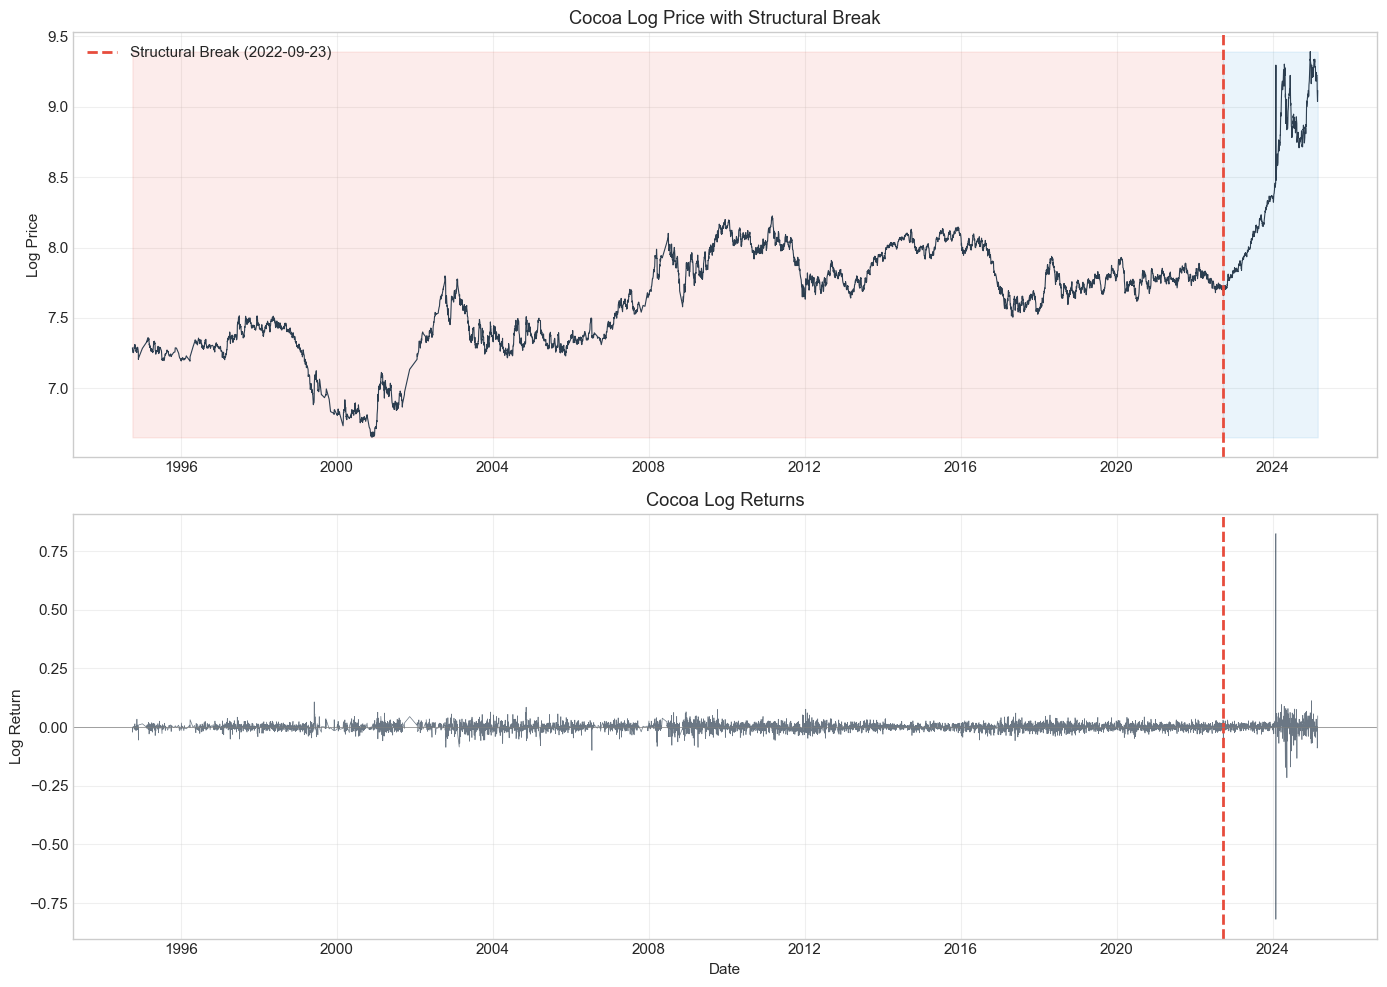
\includegraphics[keepaspectratio]{WLL_Cocoa_Experiment final_files/figure-pdf/cell-6-output-2.png}}

\begin{verbatim}

Summary Statistics by Regime:
  Pre-break  - Mean: 0.000075, Std: 0.015553, N: 6116
  Post-break - Mean: 0.002491, Std: 0.071729, N: 618
\end{verbatim}

\subsubsection{Methodology: Mohr-Selk
(2020)}\label{methodology-mohr-selk-2020}

We use the Mohr-Selk (2020) detector to locate the structural break.
Steps are simple: (1) pick a pilot bandwidth with MFV for a local linear
fit, (2) fit the pilot mean and take residuals, (3) scan candidate break
points over a trimmed sample and choose the one with the largest KS-type
statistic. The series is treated as strong mixing within each regime. In
practice here, the detector lands on break index 6117 (2022-09-23),
matching the configured break date.

\begin{Shaded}
\begin{Highlighting}[]
\CommentTok{\# Structural Break Detection using Mohr{-}Selk (2020) Method}
\ImportTok{from}\NormalTok{ cocoa.experiments.break\_detection }\ImportTok{import}\NormalTok{ estimate\_break\_mohr\_ll}
\ImportTok{from}\NormalTok{ cocoa.models.np\_regime }\ImportTok{import}\NormalTok{ NPRegimeModel}
\ImportTok{from}\NormalTok{ cocoa.models.np\_kernels }\ImportTok{import}\NormalTok{ GaussianKernel}
\ImportTok{from}\NormalTok{ cocoa.models.np\_engines }\ImportTok{import}\NormalTok{ LocalPolynomialEngine}
\ImportTok{from}\NormalTok{ cocoa.models.bandwidth }\ImportTok{import}\NormalTok{ create\_precentered\_grid}
\ImportTok{from}\NormalTok{ functools }\ImportTok{import}\NormalTok{ partial}

\BuiltInTok{print}\NormalTok{(}\StringTok{\textquotesingle{}Running Mohr{-}Selk (2020) Break Detection...\textquotesingle{}}\NormalTok{)}
\BuiltInTok{print}\NormalTok{(}\StringTok{\textquotesingle{}=\textquotesingle{}}\OperatorTok{*}\DecValTok{60}\NormalTok{)}

\CommentTok{\# Use config from assets}
\NormalTok{FEATURE\_COLS }\OperatorTok{=}\NormalTok{ DEFAULT\_FEATURE\_COLS.copy()}
\NormalTok{TARGET\_COL }\OperatorTok{=}\NormalTok{ DEFAULT\_TARGET\_COL}

\CommentTok{\# Prepare data for break detection (full training sample)}
\NormalTok{train\_mask\_full }\OperatorTok{=}\NormalTok{ df[}\StringTok{\textquotesingle{}date\textquotesingle{}}\NormalTok{] }\OperatorTok{\textless{}}\NormalTok{ pd.to\_datetime(OOS\_START\_DATE)}
\NormalTok{X\_train\_break }\OperatorTok{=}\NormalTok{ df.loc[train\_mask\_full, FEATURE\_COLS].values}
\NormalTok{y\_train\_break }\OperatorTok{=}\NormalTok{ df.loc[train\_mask\_full, TARGET\_COL].values}
\NormalTok{dates\_train }\OperatorTok{=}\NormalTok{ df.loc[train\_mask\_full, }\StringTok{\textquotesingle{}date\textquotesingle{}}\NormalTok{].values}

\NormalTok{T\_break, d\_break }\OperatorTok{=}\NormalTok{ X\_train\_break.shape}
\BuiltInTok{print}\NormalTok{(}\SpecialStringTok{f\textquotesingle{}Sample size for break detection: T = }\SpecialCharTok{\{}\NormalTok{T\_break}\SpecialCharTok{\}}\SpecialStringTok{\textquotesingle{}}\NormalTok{)}
\BuiltInTok{print}\NormalTok{(}\SpecialStringTok{f\textquotesingle{}Dimension: d = }\SpecialCharTok{\{}\NormalTok{d\_break}\SpecialCharTok{\}}\SpecialStringTok{\textquotesingle{}}\NormalTok{)}

\CommentTok{\# Step 1: Select pilot bandwidth via MFV}
\BuiltInTok{print}\NormalTok{(}\StringTok{\textquotesingle{}}\CharTok{\textbackslash{}n}\StringTok{Step 1: Selecting pilot bandwidth via MFV cross{-}validation...\textquotesingle{}}\NormalTok{)}
\NormalTok{pilot\_kernel }\OperatorTok{=}\NormalTok{ GaussianKernel()}
\NormalTok{pilot\_engine }\OperatorTok{=}\NormalTok{ LocalPolynomialEngine(order}\OperatorTok{=}\DecValTok{1}\NormalTok{, use\_gpu}\OperatorTok{=}\VariableTok{True}\NormalTok{)}
\NormalTok{pilot\_bandwidth\_grid }\OperatorTok{=}\NormalTok{ create\_precentered\_grid(T}\OperatorTok{=}\NormalTok{T\_break, d}\OperatorTok{=}\NormalTok{d\_break)}

\CommentTok{\# Use MFV to find optimal pilot bandwidth}
\NormalTok{mfv\_pilot }\OperatorTok{=}\NormalTok{ MFVValidator(Q}\OperatorTok{=}\NormalTok{Q\_VALUE)}
\NormalTok{pilot\_param\_grid }\OperatorTok{=}\NormalTok{ [}
\NormalTok{    \{}\StringTok{\textquotesingle{}kernel\textquotesingle{}}\NormalTok{: pilot\_kernel, }\StringTok{\textquotesingle{}local\_engine\textquotesingle{}}\NormalTok{: pilot\_engine, }\StringTok{\textquotesingle{}bandwidth\textquotesingle{}}\NormalTok{: h\}}
    \ControlFlowTok{for}\NormalTok{ h }\KeywordTok{in}\NormalTok{ pilot\_bandwidth\_grid}
\NormalTok{]}

\NormalTok{X\_train\_break\_df }\OperatorTok{=}\NormalTok{ pd.DataFrame(X\_train\_break, columns}\OperatorTok{=}\NormalTok{FEATURE\_COLS)}
\NormalTok{y\_train\_break\_s }\OperatorTok{=}\NormalTok{ pd.Series(y\_train\_break)}

\NormalTok{best\_pilot\_params, best\_pilot\_mse, \_ }\OperatorTok{=}\NormalTok{ mfv\_pilot.grid\_search(}
\NormalTok{    model\_class}\OperatorTok{=}\NormalTok{NPRegimeModel,}
\NormalTok{    X\_train}\OperatorTok{=}\NormalTok{X\_train\_break\_df,}
\NormalTok{    y\_train}\OperatorTok{=}\NormalTok{y\_train\_break\_s,}
\NormalTok{    param\_grid}\OperatorTok{=}\NormalTok{pilot\_param\_grid,}
\NormalTok{    verbose}\OperatorTok{=}\VariableTok{False}
\NormalTok{)}
\NormalTok{pilot\_h }\OperatorTok{=}\NormalTok{ best\_pilot\_params[}\StringTok{\textquotesingle{}bandwidth\textquotesingle{}}\NormalTok{]}
\BuiltInTok{print}\NormalTok{(}\SpecialStringTok{f\textquotesingle{}  Selected pilot bandwidth: h = }\SpecialCharTok{\{}\NormalTok{pilot\_h}\SpecialCharTok{:.4f\}}\SpecialStringTok{\textquotesingle{}}\NormalTok{)}
\BuiltInTok{print}\NormalTok{(}\SpecialStringTok{f\textquotesingle{}  Pilot MFV MSE: }\SpecialCharTok{\{}\NormalTok{best\_pilot\_mse}\SpecialCharTok{:.6f\}}\SpecialStringTok{\textquotesingle{}}\NormalTok{)}

\CommentTok{\# Step 2: Compute pilot estimates}
\BuiltInTok{print}\NormalTok{(}\StringTok{\textquotesingle{}}\CharTok{\textbackslash{}n}\StringTok{Step 2: Computing pilot estimates...\textquotesingle{}}\NormalTok{)}
\NormalTok{m\_hat }\OperatorTok{=}\NormalTok{ pilot\_engine.fit(}
\NormalTok{    X\_train\_break\_df, y\_train\_break\_s,}
\NormalTok{    X\_train\_break\_df, pilot\_h, pilot\_kernel}
\NormalTok{)}
\BuiltInTok{print}\NormalTok{(}\SpecialStringTok{f\textquotesingle{}  Pilot estimates computed for }\SpecialCharTok{\{}\BuiltInTok{len}\NormalTok{(m\_hat)}\SpecialCharTok{\}}\SpecialStringTok{ observations\textquotesingle{}}\NormalTok{)}

\CommentTok{\# Step 3: Estimate break date}
\BuiltInTok{print}\NormalTok{(}\StringTok{\textquotesingle{}}\CharTok{\textbackslash{}n}\StringTok{Step 3: Estimating break date via KS functional maximization...\textquotesingle{}}\NormalTok{)}
\NormalTok{T1\_hat }\OperatorTok{=}\NormalTok{ estimate\_break\_mohr\_ll(}
\NormalTok{    y}\OperatorTok{=}\NormalTok{y\_train\_break,}
\NormalTok{    X}\OperatorTok{=}\NormalTok{X\_train\_break,}
\NormalTok{    m\_hat}\OperatorTok{=}\NormalTok{m\_hat,}
\NormalTok{    trim\_frac}\OperatorTok{=}\FloatTok{0.05}  \CommentTok{\# Trim 5\% from each end}
\NormalTok{)}

\NormalTok{detected\_break\_date }\OperatorTok{=}\NormalTok{ dates\_train[T1\_hat }\OperatorTok{{-}} \DecValTok{1}\NormalTok{]  }\CommentTok{\# Convert to 0{-}based for indexing}
\NormalTok{detected\_break\_date\_str }\OperatorTok{=}\NormalTok{ pd.Timestamp(detected\_break\_date).strftime(}\StringTok{\textquotesingle{}\%Y{-}\%m{-}}\SpecialCharTok{\%d}\StringTok{\textquotesingle{}}\NormalTok{)}

\BuiltInTok{print}\NormalTok{(}\SpecialStringTok{f\textquotesingle{}}\CharTok{\textbackslash{}n}\SpecialStringTok{Results:\textquotesingle{}}\NormalTok{)}
\BuiltInTok{print}\NormalTok{(}\SpecialStringTok{f\textquotesingle{}  Estimated break index (1{-}based): }\SpecialCharTok{\{}\NormalTok{T1\_hat}\SpecialCharTok{\}}\SpecialStringTok{\textquotesingle{}}\NormalTok{)}
\BuiltInTok{print}\NormalTok{(}\SpecialStringTok{f\textquotesingle{}  Estimated break date: }\SpecialCharTok{\{}\NormalTok{detected\_break\_date\_str}\SpecialCharTok{\}}\SpecialStringTok{\textquotesingle{}}\NormalTok{)}
\BuiltInTok{print}\NormalTok{(}\SpecialStringTok{f\textquotesingle{}  Configured break index: }\SpecialCharTok{\{}\NormalTok{BREAK\_ID\_ONE\_BASED}\SpecialCharTok{\}}\SpecialStringTok{\textquotesingle{}}\NormalTok{)}
\BuiltInTok{print}\NormalTok{(}\SpecialStringTok{f\textquotesingle{}  Configured break date: }\SpecialCharTok{\{}\NormalTok{BREAK\_DATE}\SpecialCharTok{.}\NormalTok{strftime(}\StringTok{"\%Y{-}\%m{-}}\SpecialCharTok{\%d}\StringTok{"}\NormalTok{)}\SpecialCharTok{\}}\SpecialStringTok{\textquotesingle{}}\NormalTok{)}
\end{Highlighting}
\end{Shaded}

\begin{verbatim}
Running Mohr-Selk (2020) Break Detection...
============================================================
Sample size for break detection: T = 6694
Dimension: d = 1

Step 1: Selecting pilot bandwidth via MFV cross-validation...
LocalPolynomialEngine will use device: cuda
Creating bandwidth grid with T=6694, d=1
Generated bandwidth grid: [0.01717366 0.02864739 0.04778673 0.07971307 0.13296941 0.22180635
 0.36999529 0.61718934 1.02953386 1.71736599]
Set block size to 1338 for training length 6694 and Q=4.
  Selected pilot bandwidth: h = 1.7174
  Pilot MFV MSE: 0.000813

Step 2: Computing pilot estimates...
  Pilot estimates computed for 6694 observations

Step 3: Estimating break date via KS functional maximization...

Results:
  Estimated break index (1-based): 6117
  Estimated break date: 2022-09-23
  Configured break index: 6117
  Configured break date: 2022-09-23
\end{verbatim}

\begin{Shaded}
\begin{Highlighting}[]
\ImportTok{from}\NormalTok{ cocoa.experiments.run\_np\_combo\_cv }\ImportTok{import}\NormalTok{ gamma\_break\_grid}


\NormalTok{detected\_break }\OperatorTok{=} \DecValTok{6117}  \CommentTok{\# from Mohr{-}Selk step}
\NormalTok{df\_gamma }\OperatorTok{=}\NormalTok{ gamma\_break\_grid(start\_index}\OperatorTok{=}\NormalTok{detected\_break }\OperatorTok{{-}} \DecValTok{3}\NormalTok{,}
\NormalTok{                              end\_index}\OperatorTok{=}\NormalTok{detected\_break }\OperatorTok{+} \DecValTok{3}\NormalTok{,}
\NormalTok{                              jump\_size}\OperatorTok{=}\DecValTok{1}\NormalTok{,}
\NormalTok{                              save\_plots}\OperatorTok{=}\VariableTok{True}\NormalTok{)}

\BuiltInTok{print}\NormalTok{(df\_gamma)}
\end{Highlighting}
\end{Shaded}

\begin{verbatim}
LocalPolynomialEngine will use device: cuda
Instantiated runner for NP_LL_Combo. Results will not be saved.
Structural break date identified: 2022-09-20
Full train/CV size: 6694, OOS test size: 40

--- (1/3) Tuning bandwidth for PRE-break model ---
Creating bandwidth grid with T=6113, d=1
Generated bandwidth grid: [0.01748836 0.02917235 0.0486624  0.08117378 0.13540603 0.22587087
 0.37677533 0.62849912 1.04839973 1.74883615]
Set block size to 1222 for training length 6113 and Q=4.
Best bandwidth for PRE-break model: 1.7488

--- (2/3) Tuning bandwidth for POST-break model ---
Creating bandwidth grid with T=581, d=1
Generated bandwidth grid: [0.02800043 0.04670754 0.07791287 0.1299665  0.2167972  0.36163952
 0.60325108 1.00628345 1.67858196 2.80004347]
Set block size to 116 for training length 581 and Q=4.
Best bandwidth for POST-break model: 2.8000

--- (3/3) Tuning gamma for Convex Combination model ---
Set block size to 116 for training length 581 and Q=4.
  Gamma: 0.00, MFV MSE: 0.006723
  Gamma: 0.05, MFV MSE: 0.006722
  Gamma: 0.10, MFV MSE: 0.006722
  Gamma: 0.15, MFV MSE: 0.006722
  Gamma: 0.20, MFV MSE: 0.006721
  Gamma: 0.25, MFV MSE: 0.006722
  Gamma: 0.30, MFV MSE: 0.006722
  Gamma: 0.35, MFV MSE: 0.006722
  Gamma: 0.40, MFV MSE: 0.006723
  Gamma: 0.45, MFV MSE: 0.006723
  Gamma: 0.50, MFV MSE: 0.006724
  Gamma: 0.55, MFV MSE: 0.006725
  Gamma: 0.60, MFV MSE: 0.006727
  Gamma: 0.65, MFV MSE: 0.006728
  Gamma: 0.70, MFV MSE: 0.006730
  Gamma: 0.75, MFV MSE: 0.006731
  Gamma: 0.80, MFV MSE: 0.006733
  Gamma: 0.85, MFV MSE: 0.006735
  Gamma: 0.90, MFV MSE: 0.006737
  Gamma: 0.95, MFV MSE: 0.006740
  Gamma: 1.00, MFV MSE: 0.006742
Best gamma: 0.20 (MFV MSE: 0.006721)

--- Skipping Bias-Variance Decomposition ---
Successfully completed run for NP_LL_Combo (without saving artifacts).
LocalPolynomialEngine will use device: cuda
Instantiated runner for NP_LL_Combo. Results will not be saved.
Structural break date identified: 2022-09-21
Full train/CV size: 6694, OOS test size: 40

--- (1/3) Tuning bandwidth for PRE-break model ---
Creating bandwidth grid with T=6114, d=1
Generated bandwidth grid: [0.01748779 0.02917139 0.04866081 0.08117113 0.1354016  0.22586348
 0.376763   0.62847856 1.04836543 1.74877893]
Set block size to 1222 for training length 6114 and Q=4.
Best bandwidth for PRE-break model: 1.7488

--- (2/3) Tuning bandwidth for POST-break model ---
Creating bandwidth grid with T=580, d=1
Generated bandwidth grid: [0.02801008 0.04672364 0.07793972 0.13001129 0.2168719  0.36176414
 0.60345895 1.0066302  1.67916038 2.80100834]
Set block size to 116 for training length 580 and Q=4.
Best bandwidth for POST-break model: 2.8010

--- (3/3) Tuning gamma for Convex Combination model ---
Set block size to 116 for training length 580 and Q=4.
  Gamma: 0.00, MFV MSE: 0.006723
  Gamma: 0.05, MFV MSE: 0.006723
  Gamma: 0.10, MFV MSE: 0.006722
  Gamma: 0.15, MFV MSE: 0.006722
  Gamma: 0.20, MFV MSE: 0.006722
  Gamma: 0.25, MFV MSE: 0.006722
  Gamma: 0.30, MFV MSE: 0.006722
  Gamma: 0.35, MFV MSE: 0.006723
  Gamma: 0.40, MFV MSE: 0.006723
  Gamma: 0.45, MFV MSE: 0.006724
  Gamma: 0.50, MFV MSE: 0.006725
  Gamma: 0.55, MFV MSE: 0.006726
  Gamma: 0.60, MFV MSE: 0.006727
  Gamma: 0.65, MFV MSE: 0.006728
  Gamma: 0.70, MFV MSE: 0.006730
  Gamma: 0.75, MFV MSE: 0.006731
  Gamma: 0.80, MFV MSE: 0.006733
  Gamma: 0.85, MFV MSE: 0.006735
  Gamma: 0.90, MFV MSE: 0.006737
  Gamma: 0.95, MFV MSE: 0.006740
  Gamma: 1.00, MFV MSE: 0.006742
Best gamma: 0.20 (MFV MSE: 0.006722)

--- Skipping Bias-Variance Decomposition ---
Successfully completed run for NP_LL_Combo (without saving artifacts).
LocalPolynomialEngine will use device: cuda
Instantiated runner for NP_LL_Combo. Results will not be saved.
Structural break date identified: 2022-09-22
Full train/CV size: 6694, OOS test size: 40

--- (1/3) Tuning bandwidth for PRE-break model ---
Creating bandwidth grid with T=6115, d=1
Generated bandwidth grid: [0.01748722 0.02917044 0.04865922 0.08116847 0.13539717 0.2258561
 0.37675068 0.62845801 1.04833114 1.74872173]
Set block size to 1223 for training length 6115 and Q=4.
Best bandwidth for PRE-break model: 1.7487

--- (2/3) Tuning bandwidth for POST-break model ---
Creating bandwidth grid with T=579, d=1
Generated bandwidth grid: [0.02801975 0.04673976 0.07796662 0.13005617 0.21694676 0.36188901
 0.60366726 1.00697768 1.67974    2.8019752 ]
Set block size to 115 for training length 579 and Q=4.
Best bandwidth for POST-break model: 2.8020

--- (3/3) Tuning gamma for Convex Combination model ---
Set block size to 115 for training length 579 and Q=4.
  Gamma: 0.00, MFV MSE: 0.007149
  Gamma: 0.05, MFV MSE: 0.007110
  Gamma: 0.10, MFV MSE: 0.007073
  Gamma: 0.15, MFV MSE: 0.007038
  Gamma: 0.20, MFV MSE: 0.007006
  Gamma: 0.25, MFV MSE: 0.006976
  Gamma: 0.30, MFV MSE: 0.006949
  Gamma: 0.35, MFV MSE: 0.006923
  Gamma: 0.40, MFV MSE: 0.006900
  Gamma: 0.45, MFV MSE: 0.006879
  Gamma: 0.50, MFV MSE: 0.006861
  Gamma: 0.55, MFV MSE: 0.006844
  Gamma: 0.60, MFV MSE: 0.006830
  Gamma: 0.65, MFV MSE: 0.006819
  Gamma: 0.70, MFV MSE: 0.006809
  Gamma: 0.75, MFV MSE: 0.006802
  Gamma: 0.80, MFV MSE: 0.006797
  Gamma: 0.85, MFV MSE: 0.006794
  Gamma: 0.90, MFV MSE: 0.006794
  Gamma: 0.95, MFV MSE: 0.006796
  Gamma: 1.00, MFV MSE: 0.006800
Best gamma: 0.90 (MFV MSE: 0.006794)

--- Skipping Bias-Variance Decomposition ---
Successfully completed run for NP_LL_Combo (without saving artifacts).
LocalPolynomialEngine will use device: cuda
Instantiated runner for NP_LL_Combo. Results will not be saved.
Structural break date identified: 2022-09-23
Full train/CV size: 6694, OOS test size: 40

--- (1/3) Tuning bandwidth for PRE-break model ---
Creating bandwidth grid with T=6116, d=1
Generated bandwidth grid: [0.01748665 0.02916948 0.04865763 0.08116582 0.13539275 0.22584871
 0.37673836 0.62843745 1.04829685 1.74866455]
Set block size to 1223 for training length 6116 and Q=4.
Best bandwidth for PRE-break model: 1.7487

--- (2/3) Tuning bandwidth for POST-break model ---
Creating bandwidth grid with T=578, d=1
Generated bandwidth grid: [0.02802944 0.04675593 0.07799358 0.13010114 0.21702178 0.36201415
 0.60387599 1.00732587 1.68032083 2.80294407]
Set block size to 115 for training length 578 and Q=4.
Best bandwidth for POST-break model: 2.8029

--- (3/3) Tuning gamma for Convex Combination model ---
Set block size to 115 for training length 578 and Q=4.
  Gamma: 0.00, MFV MSE: 0.007153
  Gamma: 0.05, MFV MSE: 0.007114
  Gamma: 0.10, MFV MSE: 0.007076
  Gamma: 0.15, MFV MSE: 0.007041
  Gamma: 0.20, MFV MSE: 0.007008
  Gamma: 0.25, MFV MSE: 0.006978
  Gamma: 0.30, MFV MSE: 0.006949
  Gamma: 0.35, MFV MSE: 0.006924
  Gamma: 0.40, MFV MSE: 0.006900
  Gamma: 0.45, MFV MSE: 0.006879
  Gamma: 0.50, MFV MSE: 0.006860
  Gamma: 0.55, MFV MSE: 0.006844
  Gamma: 0.60, MFV MSE: 0.006829
  Gamma: 0.65, MFV MSE: 0.006818
  Gamma: 0.70, MFV MSE: 0.006808
  Gamma: 0.75, MFV MSE: 0.006801
  Gamma: 0.80, MFV MSE: 0.006796
  Gamma: 0.85, MFV MSE: 0.006794
  Gamma: 0.90, MFV MSE: 0.006793
  Gamma: 0.95, MFV MSE: 0.006796
  Gamma: 1.00, MFV MSE: 0.006800
Best gamma: 0.90 (MFV MSE: 0.006793)

--- Skipping Bias-Variance Decomposition ---
Successfully completed run for NP_LL_Combo (without saving artifacts).
LocalPolynomialEngine will use device: cuda
Instantiated runner for NP_LL_Combo. Results will not be saved.
Structural break date identified: 2022-09-26
Full train/CV size: 6694, OOS test size: 40

--- (1/3) Tuning bandwidth for PRE-break model ---
Creating bandwidth grid with T=6117, d=1
Generated bandwidth grid: [0.01748607 0.02916853 0.04865604 0.08116316 0.13538832 0.22584133
 0.37672604 0.62841691 1.04826258 1.74860737]
Set block size to 1223 for training length 6117 and Q=4.
Best bandwidth for PRE-break model: 1.7486

--- (2/3) Tuning bandwidth for POST-break model ---
Creating bandwidth grid with T=577, d=1
Generated bandwidth grid: [0.02803915 0.04677212 0.0780206  0.1301462  0.21709695 0.36213954
 0.60408517 1.00767479 1.68090286 2.80391496]
Set block size to 115 for training length 577 and Q=4.
Best bandwidth for POST-break model: 2.8039

--- (3/3) Tuning gamma for Convex Combination model ---
Set block size to 115 for training length 577 and Q=4.
  Gamma: 0.00, MFV MSE: 0.007158
  Gamma: 0.05, MFV MSE: 0.007119
  Gamma: 0.10, MFV MSE: 0.007081
  Gamma: 0.15, MFV MSE: 0.007046
  Gamma: 0.20, MFV MSE: 0.007014
  Gamma: 0.25, MFV MSE: 0.006983
  Gamma: 0.30, MFV MSE: 0.006955
  Gamma: 0.35, MFV MSE: 0.006929
  Gamma: 0.40, MFV MSE: 0.006906
  Gamma: 0.45, MFV MSE: 0.006885
  Gamma: 0.50, MFV MSE: 0.006866
  Gamma: 0.55, MFV MSE: 0.006849
  Gamma: 0.60, MFV MSE: 0.006834
  Gamma: 0.65, MFV MSE: 0.006822
  Gamma: 0.70, MFV MSE: 0.006812
  Gamma: 0.75, MFV MSE: 0.006805
  Gamma: 0.80, MFV MSE: 0.006799
  Gamma: 0.85, MFV MSE: 0.006796
  Gamma: 0.90, MFV MSE: 0.006795
  Gamma: 0.95, MFV MSE: 0.006797
  Gamma: 1.00, MFV MSE: 0.006800
Best gamma: 0.90 (MFV MSE: 0.006795)

--- Skipping Bias-Variance Decomposition ---
Successfully completed run for NP_LL_Combo (without saving artifacts).
LocalPolynomialEngine will use device: cuda
Instantiated runner for NP_LL_Combo. Results will not be saved.
Structural break date identified: 2022-09-27
Full train/CV size: 6694, OOS test size: 40

--- (1/3) Tuning bandwidth for PRE-break model ---
Creating bandwidth grid with T=6118, d=1
Generated bandwidth grid: [0.0174855  0.02916758 0.04865445 0.08116051 0.13538389 0.22583394
 0.37671372 0.62839636 1.04822831 1.7485502 ]
Set block size to 1223 for training length 6118 and Q=4.
Best bandwidth for PRE-break model: 1.7486

--- (2/3) Tuning bandwidth for POST-break model ---
Creating bandwidth grid with T=576, d=1
Generated bandwidth grid: [0.02804888 0.04678835 0.07804767 0.13019136 0.21717228 0.3622652
 0.60429477 1.00802443 1.6814861  2.80488786]
Set block size to 115 for training length 576 and Q=4.
Best bandwidth for POST-break model: 2.8049

--- (3/3) Tuning gamma for Convex Combination model ---
Set block size to 115 for training length 576 and Q=4.
  Gamma: 0.00, MFV MSE: 0.007161
  Gamma: 0.05, MFV MSE: 0.007121
  Gamma: 0.10, MFV MSE: 0.007084
  Gamma: 0.15, MFV MSE: 0.007049
  Gamma: 0.20, MFV MSE: 0.007015
  Gamma: 0.25, MFV MSE: 0.006985
  Gamma: 0.30, MFV MSE: 0.006956
  Gamma: 0.35, MFV MSE: 0.006930
  Gamma: 0.40, MFV MSE: 0.006906
  Gamma: 0.45, MFV MSE: 0.006885
  Gamma: 0.50, MFV MSE: 0.006866
  Gamma: 0.55, MFV MSE: 0.006849
  Gamma: 0.60, MFV MSE: 0.006834
  Gamma: 0.65, MFV MSE: 0.006822
  Gamma: 0.70, MFV MSE: 0.006812
  Gamma: 0.75, MFV MSE: 0.006804
  Gamma: 0.80, MFV MSE: 0.006799
  Gamma: 0.85, MFV MSE: 0.006796
  Gamma: 0.90, MFV MSE: 0.006795
  Gamma: 0.95, MFV MSE: 0.006796
  Gamma: 1.00, MFV MSE: 0.006800
Best gamma: 0.90 (MFV MSE: 0.006795)

--- Skipping Bias-Variance Decomposition ---
Successfully completed run for NP_LL_Combo (without saving artifacts).
LocalPolynomialEngine will use device: cuda
Instantiated runner for NP_LL_Combo. Results will not be saved.
Structural break date identified: 2022-09-28
Full train/CV size: 6694, OOS test size: 40

--- (1/3) Tuning bandwidth for PRE-break model ---
Creating bandwidth grid with T=6119, d=1
Generated bandwidth grid: [0.01748493 0.02916662 0.04865286 0.08115786 0.13537947 0.22582656
 0.37670141 0.62837582 1.04819404 1.74849305]
Set block size to 1223 for training length 6119 and Q=4.
Best bandwidth for PRE-break model: 1.7485

--- (2/3) Tuning bandwidth for POST-break model ---
Creating bandwidth grid with T=575, d=1
Generated bandwidth grid: [0.02805863 0.04680461 0.0780748  0.13023661 0.21724777 0.36239112
 0.60450481 1.00837481 1.68207056 2.8058628 ]
Set block size to 115 for training length 575 and Q=4.
Best bandwidth for POST-break model: 2.8059

--- (3/3) Tuning gamma for Convex Combination model ---
Set block size to 115 for training length 575 and Q=4.
  Gamma: 0.00, MFV MSE: 0.007167
  Gamma: 0.05, MFV MSE: 0.007126
  Gamma: 0.10, MFV MSE: 0.007088
  Gamma: 0.15, MFV MSE: 0.007052
  Gamma: 0.20, MFV MSE: 0.007019
  Gamma: 0.25, MFV MSE: 0.006987
  Gamma: 0.30, MFV MSE: 0.006959
  Gamma: 0.35, MFV MSE: 0.006932
  Gamma: 0.40, MFV MSE: 0.006908
  Gamma: 0.45, MFV MSE: 0.006886
  Gamma: 0.50, MFV MSE: 0.006867
  Gamma: 0.55, MFV MSE: 0.006849
  Gamma: 0.60, MFV MSE: 0.006835
  Gamma: 0.65, MFV MSE: 0.006822
  Gamma: 0.70, MFV MSE: 0.006812
  Gamma: 0.75, MFV MSE: 0.006804
  Gamma: 0.80, MFV MSE: 0.006799
  Gamma: 0.85, MFV MSE: 0.006796
  Gamma: 0.90, MFV MSE: 0.006795
  Gamma: 0.95, MFV MSE: 0.006796
  Gamma: 1.00, MFV MSE: 0.006800
Best gamma: 0.90 (MFV MSE: 0.006795)

--- Skipping Bias-Variance Decomposition ---
Successfully completed run for NP_LL_Combo (without saving artifacts).
   break_index break_date  gamma  in_sample_cv_mse oos_mse
0         6114 2022-09-20    0.2          0.006721    None
1         6115 2022-09-21    0.2          0.006722    None
2         6116 2022-09-22    0.9          0.006794    None
3         6117 2022-09-23    0.9          0.006793    None
4         6118 2022-09-26    0.9          0.006795    None
5         6119 2022-09-27    0.9          0.006795    None
6         6120 2022-09-28    0.9          0.006795    None
\end{verbatim}

\pandocbounded{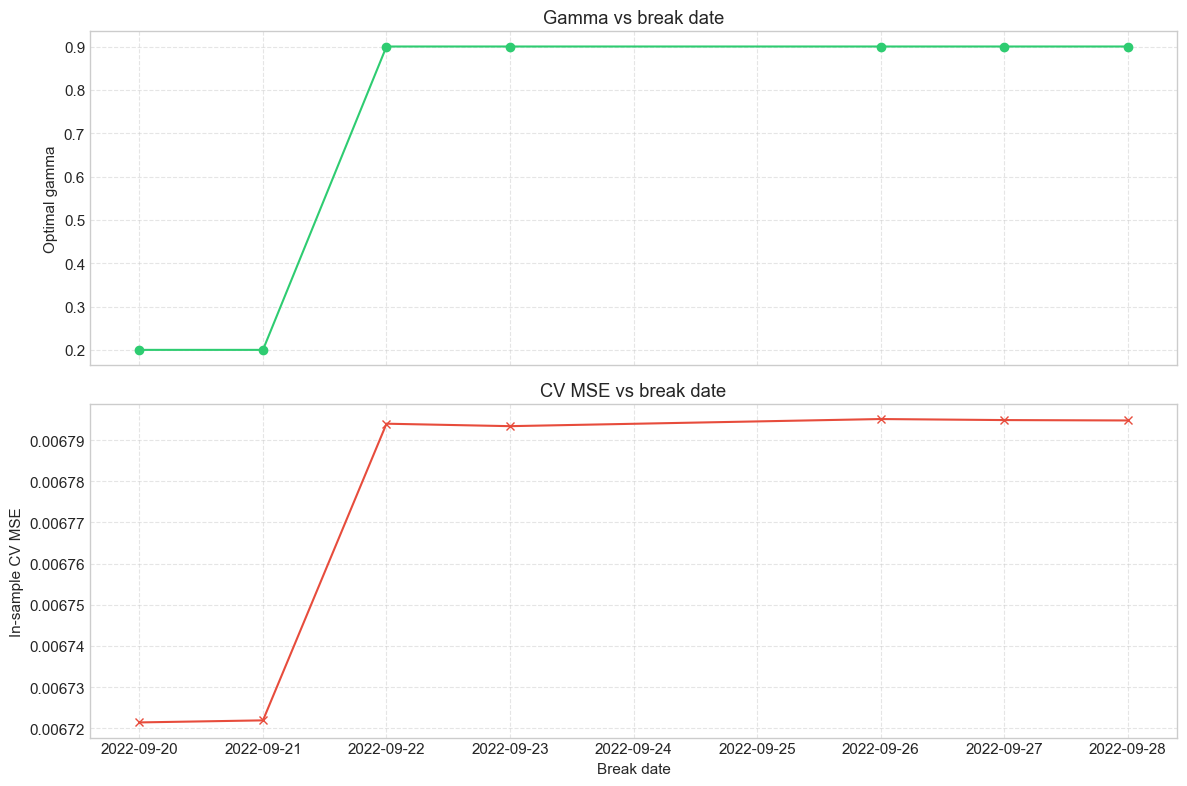
\includegraphics[keepaspectratio]{WLL_Cocoa_Experiment final_files/figure-pdf/cell-8-output-2.png}}

\begin{Shaded}
\begin{Highlighting}[]
\CommentTok{\# Visualize the detected break point}
\NormalTok{fig, axes }\OperatorTok{=}\NormalTok{ plt.subplots(}\DecValTok{2}\NormalTok{, }\DecValTok{1}\NormalTok{, figsize}\OperatorTok{=}\NormalTok{(}\DecValTok{14}\NormalTok{, }\DecValTok{10}\NormalTok{))}

\CommentTok{\# Plot 1: Log price with detected break}
\NormalTok{ax1 }\OperatorTok{=}\NormalTok{ axes[}\DecValTok{0}\NormalTok{]}
\NormalTok{ax1.plot(df[}\StringTok{\textquotesingle{}date\textquotesingle{}}\NormalTok{], df[}\StringTok{\textquotesingle{}log\_price\textquotesingle{}}\NormalTok{], color}\OperatorTok{=}\StringTok{\textquotesingle{}\#2C3E50\textquotesingle{}}\NormalTok{, linewidth}\OperatorTok{=}\FloatTok{0.8}\NormalTok{, label}\OperatorTok{=}\StringTok{\textquotesingle{}Log Price\textquotesingle{}}\NormalTok{)}
\NormalTok{ax1.axvline(x}\OperatorTok{=}\NormalTok{pd.Timestamp(detected\_break\_date), color}\OperatorTok{=}\StringTok{\textquotesingle{}\#E74C3C\textquotesingle{}}\NormalTok{, linestyle}\OperatorTok{=}\StringTok{\textquotesingle{}{-}{-}\textquotesingle{}}\NormalTok{, }
\NormalTok{            linewidth}\OperatorTok{=}\DecValTok{2}\NormalTok{, label}\OperatorTok{=}\SpecialStringTok{f\textquotesingle{}Detected Break (}\SpecialCharTok{\{}\NormalTok{detected\_break\_date\_str}\SpecialCharTok{\}}\SpecialStringTok{)\textquotesingle{}}\NormalTok{)}
\NormalTok{ax1.axvline(x}\OperatorTok{=}\NormalTok{BREAK\_DATE, color}\OperatorTok{=}\StringTok{\textquotesingle{}\#3498DB\textquotesingle{}}\NormalTok{, linestyle}\OperatorTok{=}\StringTok{\textquotesingle{}:\textquotesingle{}}\NormalTok{, }
\NormalTok{            linewidth}\OperatorTok{=}\DecValTok{2}\NormalTok{, label}\OperatorTok{=}\SpecialStringTok{f\textquotesingle{}Configured Break (}\SpecialCharTok{\{}\NormalTok{BREAK\_DATE}\SpecialCharTok{.}\NormalTok{strftime(}\StringTok{"\%Y{-}\%m{-}}\SpecialCharTok{\%d}\StringTok{"}\NormalTok{)}\SpecialCharTok{\}}\SpecialStringTok{)\textquotesingle{}}\NormalTok{)}
\NormalTok{ax1.set\_ylabel(}\StringTok{\textquotesingle{}Log Price\textquotesingle{}}\NormalTok{)}
\NormalTok{ax1.set\_title(}\StringTok{\textquotesingle{}Structural Break Detection: Mohr{-}Selk (2020) Method\textquotesingle{}}\NormalTok{)}
\NormalTok{ax1.legend(loc}\OperatorTok{=}\StringTok{\textquotesingle{}upper left\textquotesingle{}}\NormalTok{)}
\NormalTok{ax1.grid(}\VariableTok{True}\NormalTok{, alpha}\OperatorTok{=}\FloatTok{0.3}\NormalTok{)}

\CommentTok{\# Plot 2: Rolling volatility to illustrate regime change}
\NormalTok{ax2 }\OperatorTok{=}\NormalTok{ axes[}\DecValTok{1}\NormalTok{]}
\NormalTok{rolling\_vol }\OperatorTok{=}\NormalTok{ df[}\StringTok{\textquotesingle{}log\_return\textquotesingle{}}\NormalTok{].rolling(window}\OperatorTok{=}\DecValTok{60}\NormalTok{).std() }\OperatorTok{*}\NormalTok{ np.sqrt(}\DecValTok{252}\NormalTok{)  }\CommentTok{\# Annualized}
\NormalTok{ax2.plot(df[}\StringTok{\textquotesingle{}date\textquotesingle{}}\NormalTok{], rolling\_vol, color}\OperatorTok{=}\StringTok{\textquotesingle{}\#2C3E50\textquotesingle{}}\NormalTok{, linewidth}\OperatorTok{=}\FloatTok{0.8}\NormalTok{, label}\OperatorTok{=}\StringTok{\textquotesingle{}60{-}day Rolling Volatility\textquotesingle{}}\NormalTok{)}
\NormalTok{ax2.axvline(x}\OperatorTok{=}\NormalTok{pd.Timestamp(detected\_break\_date), color}\OperatorTok{=}\StringTok{\textquotesingle{}\#E74C3C\textquotesingle{}}\NormalTok{, linestyle}\OperatorTok{=}\StringTok{\textquotesingle{}{-}{-}\textquotesingle{}}\NormalTok{, linewidth}\OperatorTok{=}\DecValTok{2}\NormalTok{)}
\NormalTok{ax2.axvline(x}\OperatorTok{=}\NormalTok{BREAK\_DATE, color}\OperatorTok{=}\StringTok{\textquotesingle{}\#3498DB\textquotesingle{}}\NormalTok{, linestyle}\OperatorTok{=}\StringTok{\textquotesingle{}:\textquotesingle{}}\NormalTok{, linewidth}\OperatorTok{=}\DecValTok{2}\NormalTok{)}
\NormalTok{ax2.set\_xlabel(}\StringTok{\textquotesingle{}Date\textquotesingle{}}\NormalTok{)}
\NormalTok{ax2.set\_ylabel(}\StringTok{\textquotesingle{}Annualized Volatility\textquotesingle{}}\NormalTok{)}
\NormalTok{ax2.set\_title(}\StringTok{\textquotesingle{}Rolling Volatility (Evidence of Regime Change)\textquotesingle{}}\NormalTok{)}
\NormalTok{ax2.legend(loc}\OperatorTok{=}\StringTok{\textquotesingle{}upper left\textquotesingle{}}\NormalTok{)}
\NormalTok{ax2.grid(}\VariableTok{True}\NormalTok{, alpha}\OperatorTok{=}\FloatTok{0.3}\NormalTok{)}

\NormalTok{plt.tight\_layout()}
\NormalTok{plt.show()}

\CommentTok{\# Summary}
\BuiltInTok{print}\NormalTok{( }\StringTok{"break index is "}\NormalTok{, detected\_break,}\StringTok{"break date is "}\NormalTok{, detected\_break\_date\_str,}\StringTok{""}\NormalTok{)}
\end{Highlighting}
\end{Shaded}

\pandocbounded{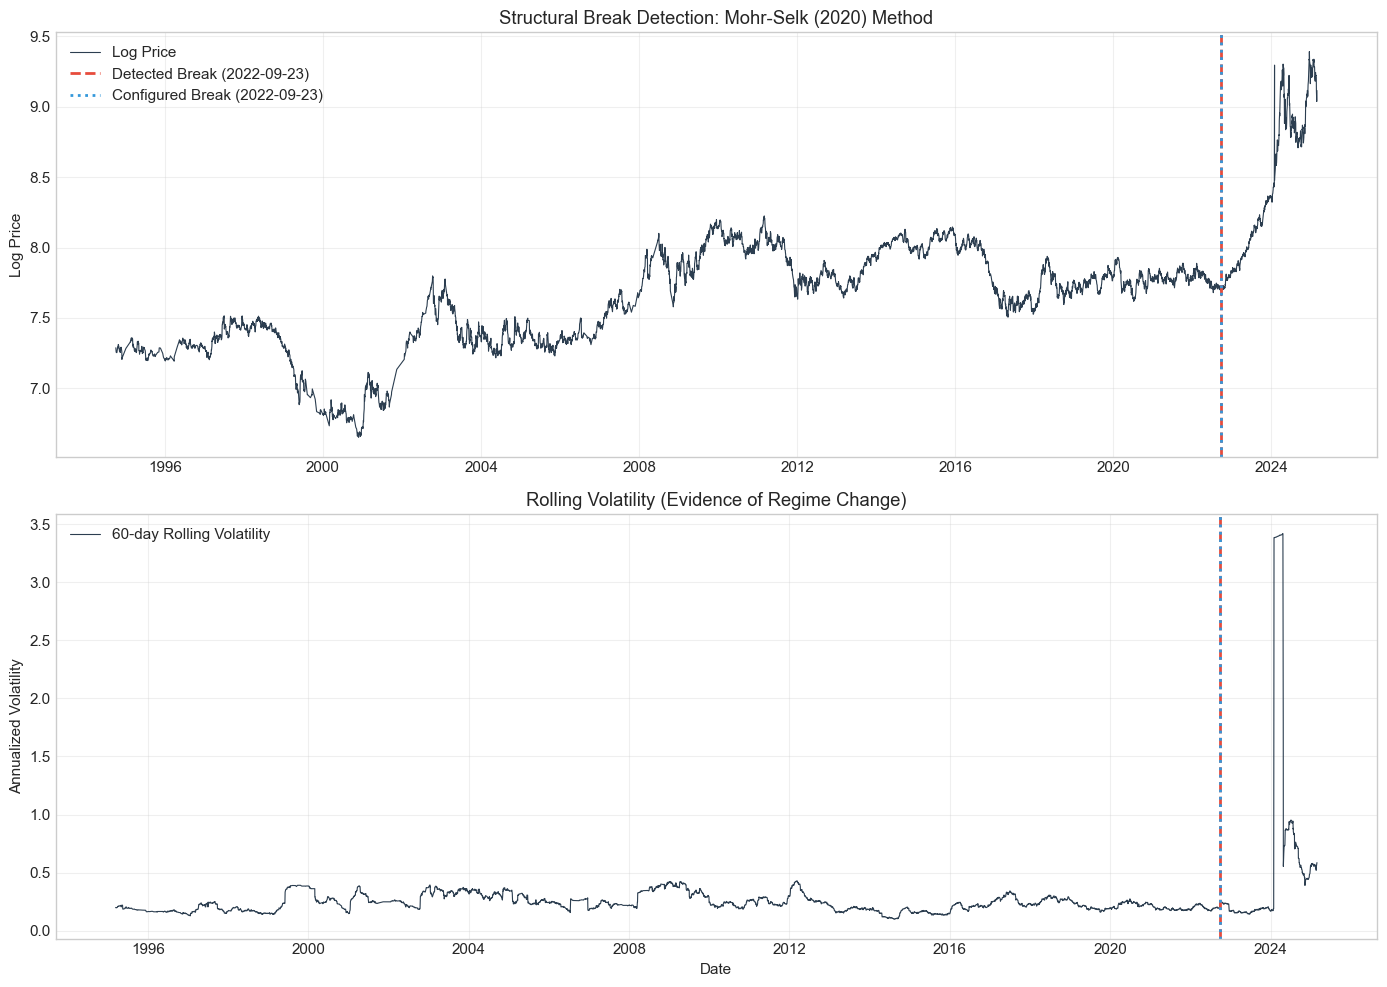
\includegraphics[keepaspectratio]{WLL_Cocoa_Experiment final_files/figure-pdf/cell-9-output-1.png}}

\begin{verbatim}
break index is  6117 break date is  2022-09-23 
\end{verbatim}

The Mohr--Selk detector flags a break at index 6117 (2022-09-23). Even
by eye the big jump feels like it climaxes in 2024 (El Niño), but a 2022
start is still plausible: it captures the earlier shift in mean/vol
driven by tightening supply conditions that lead into the 2024 spike. So
the detected break is economically interpretable as the onset of the
regime that later peaks with El Niño.

\subsection{4. Experiment Configuration}\label{experiment-configuration}

\begin{Shaded}
\begin{Highlighting}[]
\CommentTok{\# Feature and target configuration}
\NormalTok{FEATURE\_COLS }\OperatorTok{=}\NormalTok{ DEFAULT\_FEATURE\_COLS.copy()}
\NormalTok{TARGET\_COL }\OperatorTok{=}\NormalTok{ DEFAULT\_TARGET\_COL}
\NormalTok{OOS\_DATE }\OperatorTok{=}\NormalTok{ pd.to\_datetime(OOS\_START\_DATE)}

\CommentTok{\# Train/test split}
\NormalTok{train\_mask }\OperatorTok{=}\NormalTok{ df[}\StringTok{\textquotesingle{}date\textquotesingle{}}\NormalTok{] }\OperatorTok{\textless{}}\NormalTok{ OOS\_DATE}
\NormalTok{test\_mask }\OperatorTok{=}\NormalTok{ df[}\StringTok{\textquotesingle{}date\textquotesingle{}}\NormalTok{] }\OperatorTok{\textgreater{}=}\NormalTok{ OOS\_DATE}

\NormalTok{X\_train\_full }\OperatorTok{=}\NormalTok{ df.loc[train\_mask, FEATURE\_COLS].reset\_index(drop}\OperatorTok{=}\VariableTok{True}\NormalTok{)}
\NormalTok{y\_train\_full }\OperatorTok{=}\NormalTok{ df.loc[train\_mask, TARGET\_COL].reset\_index(drop}\OperatorTok{=}\VariableTok{True}\NormalTok{)}
\NormalTok{X\_test }\OperatorTok{=}\NormalTok{ df.loc[test\_mask, FEATURE\_COLS].reset\_index(drop}\OperatorTok{=}\VariableTok{True}\NormalTok{)}
\NormalTok{y\_test }\OperatorTok{=}\NormalTok{ df.loc[test\_mask, TARGET\_COL].reset\_index(drop}\OperatorTok{=}\VariableTok{True}\NormalTok{)}
\NormalTok{test\_dates }\OperatorTok{=}\NormalTok{ df.loc[test\_mask, }\StringTok{\textquotesingle{}date\textquotesingle{}}\NormalTok{].reset\_index(drop}\OperatorTok{=}\VariableTok{True}\NormalTok{)}

\CommentTok{\# Break index relative to training data}
\NormalTok{TRAIN\_BREAK\_INDEX }\OperatorTok{=} \BuiltInTok{min}\NormalTok{(BREAK\_INDEX, }\BuiltInTok{len}\NormalTok{(X\_train\_full) }\OperatorTok{{-}} \DecValTok{1}\NormalTok{)}

\BuiltInTok{print}\NormalTok{(}\StringTok{\textquotesingle{}Experiment Configuration:\textquotesingle{}}\NormalTok{)}
\BuiltInTok{print}\NormalTok{(}\SpecialStringTok{f\textquotesingle{}  Features: }\SpecialCharTok{\{}\NormalTok{FEATURE\_COLS}\SpecialCharTok{\}}\SpecialStringTok{\textquotesingle{}}\NormalTok{)}
\BuiltInTok{print}\NormalTok{(}\SpecialStringTok{f\textquotesingle{}  Target: }\SpecialCharTok{\{}\NormalTok{TARGET\_COL}\SpecialCharTok{\}}\SpecialStringTok{\textquotesingle{}}\NormalTok{)}
\BuiltInTok{print}\NormalTok{(}\SpecialStringTok{f\textquotesingle{}  Training set: }\SpecialCharTok{\{}\BuiltInTok{len}\NormalTok{(X\_train\_full)}\SpecialCharTok{:,\}}\SpecialStringTok{ observations\textquotesingle{}}\NormalTok{)}
\BuiltInTok{print}\NormalTok{(}\SpecialStringTok{f\textquotesingle{}  Test set (OOS): }\SpecialCharTok{\{}\BuiltInTok{len}\NormalTok{(X\_test)}\SpecialCharTok{:,\}}\SpecialStringTok{ observations\textquotesingle{}}\NormalTok{)}
\BuiltInTok{print}\NormalTok{(}\SpecialStringTok{f\textquotesingle{}  OOS Start: }\SpecialCharTok{\{}\NormalTok{OOS\_DATE}\SpecialCharTok{.}\NormalTok{strftime(}\StringTok{"\%Y{-}\%m{-}}\SpecialCharTok{\%d}\StringTok{"}\NormalTok{)}\SpecialCharTok{\}}\SpecialStringTok{\textquotesingle{}}\NormalTok{)}
\BuiltInTok{print}\NormalTok{(}\SpecialStringTok{f\textquotesingle{}  Break index (training): }\SpecialCharTok{\{}\NormalTok{TRAIN\_BREAK\_INDEX}\SpecialCharTok{\}}\SpecialStringTok{\textquotesingle{}}\NormalTok{)}
\BuiltInTok{print}\NormalTok{(}\SpecialStringTok{f\textquotesingle{}  MFV Folds (Q): }\SpecialCharTok{\{}\NormalTok{Q\_VALUE}\SpecialCharTok{\}}\SpecialStringTok{\textquotesingle{}}\NormalTok{)}
\end{Highlighting}
\end{Shaded}

\begin{verbatim}
Experiment Configuration:
  Features: ['log_price_lagt']
  Target: log_return_forecast_target
  Training set: 6,694 observations
  Test set (OOS): 40 observations
  OOS Start: 2025-01-02
  Break index (training): 6116
  MFV Folds (Q): 4
\end{verbatim}

\subsection{5. Model Training}\label{model-training}

\subsubsection{5.1 Non-Parametric
Benchmarks}\label{non-parametric-benchmarks}

\begin{Shaded}
\begin{Highlighting}[]
\CommentTok{\# Initialize NP components}
\NormalTok{kernel }\OperatorTok{=}\NormalTok{ EpanechnikovKernel()}
\NormalTok{local\_engine }\OperatorTok{=}\NormalTok{ LocalPolynomialEngine(order}\OperatorTok{=}\DecValTok{1}\NormalTok{, use\_gpu}\OperatorTok{=}\VariableTok{True}\NormalTok{)}

\CommentTok{\# Bandwidth grid}
\NormalTok{T\_train }\OperatorTok{=} \BuiltInTok{len}\NormalTok{(X\_train\_full)}
\NormalTok{d }\OperatorTok{=} \BuiltInTok{len}\NormalTok{(FEATURE\_COLS)}
\NormalTok{bandwidth\_grid }\OperatorTok{=}\NormalTok{ create\_precentered\_grid(T}\OperatorTok{=}\NormalTok{T\_train, d}\OperatorTok{=}\NormalTok{d, C}\OperatorTok{=}\FloatTok{1.0}\NormalTok{)}

\BuiltInTok{print}\NormalTok{(}\SpecialStringTok{f\textquotesingle{}NP Configuration:\textquotesingle{}}\NormalTok{)}
\BuiltInTok{print}\NormalTok{(}\SpecialStringTok{f\textquotesingle{}  Kernel: Epanechnikov\textquotesingle{}}\NormalTok{)}
\BuiltInTok{print}\NormalTok{(}\SpecialStringTok{f\textquotesingle{}  Local Engine: Local Linear (order=1)\textquotesingle{}}\NormalTok{)}
\BuiltInTok{print}\NormalTok{(}\SpecialStringTok{f\textquotesingle{}  Dimension: }\SpecialCharTok{\{}\NormalTok{d}\SpecialCharTok{\}}\SpecialStringTok{\textquotesingle{}}\NormalTok{)}
\BuiltInTok{print}\NormalTok{(}\SpecialStringTok{f\textquotesingle{}  Bandwidth grid: }\SpecialCharTok{\{}\BuiltInTok{len}\NormalTok{(bandwidth\_grid)}\SpecialCharTok{\}}\SpecialStringTok{ candidates\textquotesingle{}}\NormalTok{)}
\BuiltInTok{print}\NormalTok{(}\SpecialStringTok{f\textquotesingle{}  Range: [}\SpecialCharTok{\{}\NormalTok{bandwidth\_grid}\SpecialCharTok{.}\BuiltInTok{min}\NormalTok{()}\SpecialCharTok{:.4f\}}\SpecialStringTok{, }\SpecialCharTok{\{}\NormalTok{bandwidth\_grid}\SpecialCharTok{.}\BuiltInTok{max}\NormalTok{()}\SpecialCharTok{:.4f\}}\SpecialStringTok{]\textquotesingle{}}\NormalTok{)}


\KeywordTok{def}\NormalTok{ select\_bandwidth\_mfv(X\_train, y\_train, bandwidth\_grid, kernel, local\_engine, Q}\OperatorTok{=}\DecValTok{4}\NormalTok{):}
    \CommentTok{"""Select optimal bandwidth using Multi{-}Fold Forward Validation."""}
\NormalTok{    mfv }\OperatorTok{=}\NormalTok{ MFVValidator(Q}\OperatorTok{=}\NormalTok{Q)}
\NormalTok{    param\_grid }\OperatorTok{=}\NormalTok{ [}
\NormalTok{        \{}\StringTok{\textquotesingle{}kernel\textquotesingle{}}\NormalTok{: kernel, }\StringTok{\textquotesingle{}local\_engine\textquotesingle{}}\NormalTok{: local\_engine, }\StringTok{\textquotesingle{}bandwidth\textquotesingle{}}\NormalTok{: h\}}
        \ControlFlowTok{for}\NormalTok{ h }\KeywordTok{in}\NormalTok{ bandwidth\_grid}
\NormalTok{    ]}
\NormalTok{    best\_params, best\_mse, \_ }\OperatorTok{=}\NormalTok{ mfv.grid\_search(}
\NormalTok{        model\_class}\OperatorTok{=}\NormalTok{NPRegimeModel,}
\NormalTok{        X\_train}\OperatorTok{=}\NormalTok{X\_train, y\_train}\OperatorTok{=}\NormalTok{y\_train,}
\NormalTok{        param\_grid}\OperatorTok{=}\NormalTok{param\_grid, verbose}\OperatorTok{=}\VariableTok{False}
\NormalTok{    )}
    \ControlFlowTok{return}\NormalTok{ best\_params[}\StringTok{\textquotesingle{}bandwidth\textquotesingle{}}\NormalTok{], best\_mse}
\end{Highlighting}
\end{Shaded}

\begin{verbatim}
LocalPolynomialEngine will use device: cuda
Creating bandwidth grid with T=6694, d=1
Generated bandwidth grid: [0.01717366 0.02864739 0.04778673 0.07971307 0.13296941 0.22180635
 0.36999529 0.61718934 1.02953386 1.71736599]
NP Configuration:
  Kernel: Epanechnikov
  Local Engine: Local Linear (order=1)
  Dimension: 1
  Bandwidth grid: 10 candidates
  Range: [0.0172, 1.7174]
\end{verbatim}

\begin{Shaded}
\begin{Highlighting}[]
\CommentTok{\# Pre{-}Break Local Linear Model}
\BuiltInTok{print}\NormalTok{(}\StringTok{\textquotesingle{}Training Pre{-}Break Local Linear Model...\textquotesingle{}}\NormalTok{)}

\NormalTok{X\_train\_pre }\OperatorTok{=}\NormalTok{ X\_train\_full.iloc[:TRAIN\_BREAK\_INDEX]}
\NormalTok{y\_train\_pre }\OperatorTok{=}\NormalTok{ y\_train\_full.iloc[:TRAIN\_BREAK\_INDEX]}

\BuiltInTok{print}\NormalTok{(}\SpecialStringTok{f\textquotesingle{}  Training size: }\SpecialCharTok{\{}\BuiltInTok{len}\NormalTok{(X\_train\_pre)}\SpecialCharTok{:,\}}\SpecialStringTok{\textquotesingle{}}\NormalTok{)}
\BuiltInTok{print}\NormalTok{(}\StringTok{\textquotesingle{}  Selecting bandwidth via MFV...\textquotesingle{}}\NormalTok{)}

\NormalTok{bw\_pre, mse\_pre\_cv }\OperatorTok{=}\NormalTok{ select\_bandwidth\_mfv(}
\NormalTok{    X\_train\_pre, y\_train\_pre, bandwidth\_grid, kernel, local\_engine, Q}\OperatorTok{=}\NormalTok{Q\_VALUE}
\NormalTok{)}

\NormalTok{model\_pre\_ll }\OperatorTok{=}\NormalTok{ NPRegimeModel(kernel}\OperatorTok{=}\NormalTok{kernel, local\_engine}\OperatorTok{=}\NormalTok{local\_engine, bandwidth}\OperatorTok{=}\NormalTok{bw\_pre)}
\NormalTok{model\_pre\_ll.fit(X\_train\_pre, y\_train\_pre)}

\BuiltInTok{print}\NormalTok{(}\SpecialStringTok{f\textquotesingle{}  Selected bandwidth: }\SpecialCharTok{\{}\NormalTok{bw\_pre}\SpecialCharTok{:.6f\}}\SpecialStringTok{\textquotesingle{}}\NormalTok{)}
\BuiltInTok{print}\NormalTok{(}\SpecialStringTok{f\textquotesingle{}  MFV MSE: }\SpecialCharTok{\{}\NormalTok{mse\_pre\_cv}\SpecialCharTok{:.8f\}}\SpecialStringTok{\textquotesingle{}}\NormalTok{)}
\BuiltInTok{print}\NormalTok{(}\StringTok{\textquotesingle{}  Model trained.\textquotesingle{}}\NormalTok{)}
\end{Highlighting}
\end{Shaded}

\begin{verbatim}
Training Pre-Break Local Linear Model...
  Training size: 6,116
  Selecting bandwidth via MFV...
Set block size to 1223 for training length 6116 and Q=4.
  Selected bandwidth: 1.717366
  MFV MSE: 0.00025423
  Model trained.
\end{verbatim}

\begin{Shaded}
\begin{Highlighting}[]
\CommentTok{\# Post{-}Break Local Linear Model}
\BuiltInTok{print}\NormalTok{(}\StringTok{\textquotesingle{}Training Post{-}Break Local Linear Model...\textquotesingle{}}\NormalTok{)}

\NormalTok{X\_train\_post }\OperatorTok{=}\NormalTok{ X\_train\_full.iloc[TRAIN\_BREAK\_INDEX:]}
\NormalTok{y\_train\_post }\OperatorTok{=}\NormalTok{ y\_train\_full.iloc[TRAIN\_BREAK\_INDEX:]}

\BuiltInTok{print}\NormalTok{(}\SpecialStringTok{f\textquotesingle{}  Training size: }\SpecialCharTok{\{}\BuiltInTok{len}\NormalTok{(X\_train\_post)}\SpecialCharTok{:,\}}\SpecialStringTok{\textquotesingle{}}\NormalTok{)}
\BuiltInTok{print}\NormalTok{(}\StringTok{\textquotesingle{}  Selecting bandwidth via MFV...\textquotesingle{}}\NormalTok{)}

\NormalTok{bw\_post, mse\_post\_cv }\OperatorTok{=}\NormalTok{ select\_bandwidth\_mfv(}
\NormalTok{    X\_train\_post, y\_train\_post, bandwidth\_grid, kernel, local\_engine, Q}\OperatorTok{=}\NormalTok{Q\_VALUE}
\NormalTok{)}

\NormalTok{model\_post\_ll }\OperatorTok{=}\NormalTok{ NPRegimeModel(kernel}\OperatorTok{=}\NormalTok{kernel, local\_engine}\OperatorTok{=}\NormalTok{local\_engine, bandwidth}\OperatorTok{=}\NormalTok{bw\_post)}
\NormalTok{model\_post\_ll.fit(X\_train\_post, y\_train\_post)}

\BuiltInTok{print}\NormalTok{(}\SpecialStringTok{f\textquotesingle{}  Selected bandwidth: }\SpecialCharTok{\{}\NormalTok{bw\_post}\SpecialCharTok{:.6f\}}\SpecialStringTok{\textquotesingle{}}\NormalTok{)}
\BuiltInTok{print}\NormalTok{(}\SpecialStringTok{f\textquotesingle{}  MFV MSE: }\SpecialCharTok{\{}\NormalTok{mse\_post\_cv}\SpecialCharTok{:.8f\}}\SpecialStringTok{\textquotesingle{}}\NormalTok{)}
\BuiltInTok{print}\NormalTok{(}\StringTok{\textquotesingle{}  Model trained.\textquotesingle{}}\NormalTok{)}
\end{Highlighting}
\end{Shaded}

\begin{verbatim}
Training Post-Break Local Linear Model...
  Training size: 578
  Selecting bandwidth via MFV...
Set block size to 115 for training length 578 and Q=4.
  Selected bandwidth: 1.717366
  MFV MSE: 0.00767773
  Model trained.
\end{verbatim}

\begin{Shaded}
\begin{Highlighting}[]
\CommentTok{\# Weighted Local Linear Model (CGS Method)}
\BuiltInTok{print}\NormalTok{(}\StringTok{\textquotesingle{}Training Weighted Local Linear (WLL) Model...\textquotesingle{}}\NormalTok{)}

\NormalTok{mfv\_combo }\OperatorTok{=}\NormalTok{ MFVConvexComboValidator(Q}\OperatorTok{=}\NormalTok{Q\_VALUE)}
\NormalTok{gamma\_grid }\OperatorTok{=}\NormalTok{ np.linspace(}\DecValTok{0}\NormalTok{, }\DecValTok{1}\NormalTok{, }\DecValTok{21}\NormalTok{)}

\BuiltInTok{print}\NormalTok{(}\SpecialStringTok{f\textquotesingle{}  Tuning gamma via MFV...\textquotesingle{}}\NormalTok{)}
\BuiltInTok{print}\NormalTok{(}\SpecialStringTok{f\textquotesingle{}  Gamma grid: }\SpecialCharTok{\{}\BuiltInTok{len}\NormalTok{(gamma\_grid)}\SpecialCharTok{\}}\SpecialStringTok{ candidates\textquotesingle{}}\NormalTok{)}

\NormalTok{params\_pre\_np }\OperatorTok{=}\NormalTok{ \{}\StringTok{\textquotesingle{}kernel\textquotesingle{}}\NormalTok{: kernel, }\StringTok{\textquotesingle{}local\_engine\textquotesingle{}}\NormalTok{: local\_engine, }\StringTok{\textquotesingle{}bandwidth\textquotesingle{}}\NormalTok{: bw\_pre\}}
\NormalTok{params\_post\_np }\OperatorTok{=}\NormalTok{ \{}\StringTok{\textquotesingle{}kernel\textquotesingle{}}\NormalTok{: kernel, }\StringTok{\textquotesingle{}local\_engine\textquotesingle{}}\NormalTok{: local\_engine, }\StringTok{\textquotesingle{}bandwidth\textquotesingle{}}\NormalTok{: bw\_post\}}

\NormalTok{best\_gamma, best\_gamma\_mse }\OperatorTok{=}\NormalTok{ mfv\_combo.tune\_gamma(}
\NormalTok{    model\_class\_pre}\OperatorTok{=}\NormalTok{NPRegimeModel, params\_pre}\OperatorTok{=}\NormalTok{params\_pre\_np,}
\NormalTok{    model\_class\_post}\OperatorTok{=}\NormalTok{NPRegimeModel, params\_post}\OperatorTok{=}\NormalTok{params\_post\_np,}
\NormalTok{    X\_train\_full}\OperatorTok{=}\NormalTok{X\_train\_full, y\_train\_full}\OperatorTok{=}\NormalTok{y\_train\_full,}
\NormalTok{    break\_index}\OperatorTok{=}\NormalTok{TRAIN\_BREAK\_INDEX, gamma\_grid}\OperatorTok{=}\NormalTok{gamma\_grid, verbose}\OperatorTok{=}\VariableTok{False}
\NormalTok{)}

\NormalTok{model\_wll }\OperatorTok{=}\NormalTok{ NPConvexCombinationModel(}
\NormalTok{    kernel}\OperatorTok{=}\NormalTok{kernel, local\_engine}\OperatorTok{=}\NormalTok{local\_engine,}
\NormalTok{    pre\_bandwidth}\OperatorTok{=}\NormalTok{bw\_pre, post\_bandwidth}\OperatorTok{=}\NormalTok{bw\_post,}
\NormalTok{    break\_index}\OperatorTok{=}\NormalTok{TRAIN\_BREAK\_INDEX, gamma}\OperatorTok{=}\NormalTok{best\_gamma}
\NormalTok{)}
\NormalTok{model\_wll.fit(X\_train\_full, y\_train\_full)}

\BuiltInTok{print}\NormalTok{(}\SpecialStringTok{f\textquotesingle{}  Optimal gamma: }\SpecialCharTok{\{}\NormalTok{best\_gamma}\SpecialCharTok{:.4f\}}\SpecialStringTok{\textquotesingle{}}\NormalTok{)}
\BuiltInTok{print}\NormalTok{(}\SpecialStringTok{f\textquotesingle{}  Interpretation: }\SpecialCharTok{\{}\NormalTok{best\_gamma}\OperatorTok{*}\DecValTok{100}\SpecialCharTok{:.1f\}}\SpecialStringTok{\% weight on pre{-}break model\textquotesingle{}}\NormalTok{)}
\BuiltInTok{print}\NormalTok{(}\SpecialStringTok{f\textquotesingle{}  MFV MSE: }\SpecialCharTok{\{}\NormalTok{best\_gamma\_mse}\SpecialCharTok{:.8f\}}\SpecialStringTok{\textquotesingle{}}\NormalTok{)}
\BuiltInTok{print}\NormalTok{(}\StringTok{\textquotesingle{}  Model trained.\textquotesingle{}}\NormalTok{)}
\end{Highlighting}
\end{Shaded}

\begin{verbatim}
Training Weighted Local Linear (WLL) Model...
  Tuning gamma via MFV...
  Gamma grid: 21 candidates
Set block size to 115 for training length 578 and Q=4.
  Optimal gamma: 0.9500
  Interpretation: 95.0% weight on pre-break model
  MFV MSE: 0.00680709
  Model trained.
\end{verbatim}

\subsubsection{5.2 Machine Learning
Competitors}\label{machine-learning-competitors}

\begin{Shaded}
\begin{Highlighting}[]
\CommentTok{\# Random Forest}
\BuiltInTok{print}\NormalTok{(}\StringTok{\textquotesingle{}Training Random Forest...\textquotesingle{}}\NormalTok{)}

\NormalTok{rf\_param\_combinations }\OperatorTok{=}\NormalTok{ [}
    \BuiltInTok{dict}\NormalTok{(}\BuiltInTok{zip}\NormalTok{(RF\_PARAM\_GRID.keys(), v))}
    \ControlFlowTok{for}\NormalTok{ v }\KeywordTok{in}\NormalTok{ product(}\OperatorTok{*}\NormalTok{RF\_PARAM\_GRID.values())}
\NormalTok{]}

\BuiltInTok{print}\NormalTok{(}\SpecialStringTok{f\textquotesingle{}  Grid size: }\SpecialCharTok{\{}\BuiltInTok{len}\NormalTok{(rf\_param\_combinations)}\SpecialCharTok{\}}\SpecialStringTok{ combinations\textquotesingle{}}\NormalTok{)}
\BuiltInTok{print}\NormalTok{(}\StringTok{\textquotesingle{}  Running MFV hyperparameter tuning...\textquotesingle{}}\NormalTok{)}

\NormalTok{mfv\_rf }\OperatorTok{=}\NormalTok{ MFVValidator(Q}\OperatorTok{=}\NormalTok{Q\_VALUE)}
\NormalTok{best\_rf\_params, best\_rf\_mse, \_ }\OperatorTok{=}\NormalTok{ mfv\_rf.grid\_search(}
\NormalTok{    model\_class}\OperatorTok{=}\NormalTok{RFModel,}
\NormalTok{    X\_train}\OperatorTok{=}\NormalTok{X\_train\_full, y\_train}\OperatorTok{=}\NormalTok{y\_train\_full,}
\NormalTok{    param\_grid}\OperatorTok{=}\NormalTok{rf\_param\_combinations, verbose}\OperatorTok{=}\VariableTok{False}
\NormalTok{)}

\NormalTok{model\_rf }\OperatorTok{=}\NormalTok{ RFModel(}\OperatorTok{**}\NormalTok{best\_rf\_params)}
\NormalTok{model\_rf.fit(X\_train\_full, y\_train\_full)}

\BuiltInTok{print}\NormalTok{(}\SpecialStringTok{f\textquotesingle{}  Best params: }\SpecialCharTok{\{}\NormalTok{best\_rf\_params}\SpecialCharTok{\}}\SpecialStringTok{\textquotesingle{}}\NormalTok{)}
\BuiltInTok{print}\NormalTok{(}\SpecialStringTok{f\textquotesingle{}  MFV MSE: }\SpecialCharTok{\{}\NormalTok{best\_rf\_mse}\SpecialCharTok{:.8f\}}\SpecialStringTok{\textquotesingle{}}\NormalTok{)}
\BuiltInTok{print}\NormalTok{(}\StringTok{\textquotesingle{}  Model trained.\textquotesingle{}}\NormalTok{)}
\end{Highlighting}
\end{Shaded}

\begin{verbatim}
Training Random Forest...
  Grid size: 12 combinations
  Running MFV hyperparameter tuning...
Set block size to 1338 for training length 6694 and Q=4.
  Best params: {'n_estimators': 500, 'max_depth': 5, 'min_samples_leaf': 20, 'max_features': 'sqrt'}
  MFV MSE: 0.00082170
  Model trained.
\end{verbatim}

\begin{Shaded}
\begin{Highlighting}[]
\CommentTok{\# XGBoost}
\BuiltInTok{print}\NormalTok{(}\StringTok{\textquotesingle{}Training XGBoost...\textquotesingle{}}\NormalTok{)}

\NormalTok{xgb\_param\_combinations }\OperatorTok{=}\NormalTok{ [}
    \BuiltInTok{dict}\NormalTok{(}\BuiltInTok{zip}\NormalTok{(XGB\_PARAM\_GRID.keys(), v))}
    \ControlFlowTok{for}\NormalTok{ v }\KeywordTok{in}\NormalTok{ product(}\OperatorTok{*}\NormalTok{XGB\_PARAM\_GRID.values())}
\NormalTok{]}

\BuiltInTok{print}\NormalTok{(}\SpecialStringTok{f\textquotesingle{}  Grid size: }\SpecialCharTok{\{}\BuiltInTok{len}\NormalTok{(xgb\_param\_combinations)}\SpecialCharTok{\}}\SpecialStringTok{ combinations\textquotesingle{}}\NormalTok{)}
\BuiltInTok{print}\NormalTok{(}\StringTok{\textquotesingle{}  Running MFV hyperparameter tuning...\textquotesingle{}}\NormalTok{)}

\NormalTok{mfv\_xgb }\OperatorTok{=}\NormalTok{ MFVValidator(Q}\OperatorTok{=}\NormalTok{Q\_VALUE)}
\NormalTok{best\_xgb\_params, best\_xgb\_mse, \_ }\OperatorTok{=}\NormalTok{ mfv\_xgb.grid\_search(}
\NormalTok{    model\_class}\OperatorTok{=}\NormalTok{XGBModel,}
\NormalTok{    X\_train}\OperatorTok{=}\NormalTok{X\_train\_full, y\_train}\OperatorTok{=}\NormalTok{y\_train\_full,}
\NormalTok{    param\_grid}\OperatorTok{=}\NormalTok{xgb\_param\_combinations, verbose}\OperatorTok{=}\VariableTok{False}
\NormalTok{)}

\NormalTok{model\_xgb }\OperatorTok{=}\NormalTok{ XGBModel(}\OperatorTok{**}\NormalTok{best\_xgb\_params)}
\NormalTok{model\_xgb.fit(X\_train\_full, y\_train\_full)}

\BuiltInTok{print}\NormalTok{(}\SpecialStringTok{f\textquotesingle{}  Best params: }\SpecialCharTok{\{}\NormalTok{best\_xgb\_params}\SpecialCharTok{\}}\SpecialStringTok{\textquotesingle{}}\NormalTok{)}
\BuiltInTok{print}\NormalTok{(}\SpecialStringTok{f\textquotesingle{}  MFV MSE: }\SpecialCharTok{\{}\NormalTok{best\_xgb\_mse}\SpecialCharTok{:.8f\}}\SpecialStringTok{\textquotesingle{}}\NormalTok{)}
\BuiltInTok{print}\NormalTok{(}\StringTok{\textquotesingle{}  Model trained.\textquotesingle{}}\NormalTok{)}
\end{Highlighting}
\end{Shaded}

\begin{verbatim}
Training XGBoost...
  Grid size: 32 combinations
  Running MFV hyperparameter tuning...
Set block size to 1338 for training length 6694 and Q=4.
  Best params: {'n_estimators': 200, 'max_depth': 3, 'learning_rate': 0.05, 'subsample': 1.0, 'colsample_bytree': 0.7}
  MFV MSE: 0.00082941
  Model trained.
\end{verbatim}

\subsubsection{5.3 ML Extension: Weighted ML
Combinations}\label{ml-extension-weighted-ml-combinations}

\begin{Shaded}
\begin{Highlighting}[]
\CommentTok{\# Weighted RF Combo}
\BuiltInTok{print}\NormalTok{(}\StringTok{\textquotesingle{}Training Weighted RF Combo...\textquotesingle{}}\NormalTok{)}

\NormalTok{mfv\_rf\_combo }\OperatorTok{=}\NormalTok{ MFVConvexComboValidator(Q}\OperatorTok{=}\NormalTok{Q\_VALUE)}
\NormalTok{best\_gamma\_rf, \_ }\OperatorTok{=}\NormalTok{ mfv\_rf\_combo.tune\_gamma(}
\NormalTok{    model\_class\_pre}\OperatorTok{=}\NormalTok{RFModel, params\_pre}\OperatorTok{=}\NormalTok{best\_rf\_params,}
\NormalTok{    model\_class\_post}\OperatorTok{=}\NormalTok{RFModel, params\_post}\OperatorTok{=}\NormalTok{best\_rf\_params,}
\NormalTok{    X\_train\_full}\OperatorTok{=}\NormalTok{X\_train\_full, y\_train\_full}\OperatorTok{=}\NormalTok{y\_train\_full,}
\NormalTok{    break\_index}\OperatorTok{=}\NormalTok{TRAIN\_BREAK\_INDEX, gamma\_grid}\OperatorTok{=}\NormalTok{gamma\_grid, verbose}\OperatorTok{=}\VariableTok{False}
\NormalTok{)}

\NormalTok{model\_rf\_combo }\OperatorTok{=}\NormalTok{ MLConvexCombinationModel(}
\NormalTok{    model\_class}\OperatorTok{=}\NormalTok{RFModel, params\_pre}\OperatorTok{=}\NormalTok{best\_rf\_params, params\_post}\OperatorTok{=}\NormalTok{best\_rf\_params,}
\NormalTok{    break\_index}\OperatorTok{=}\NormalTok{TRAIN\_BREAK\_INDEX, gamma}\OperatorTok{=}\NormalTok{best\_gamma\_rf}
\NormalTok{)}
\NormalTok{model\_rf\_combo.fit(X\_train\_full, y\_train\_full)}
\BuiltInTok{print}\NormalTok{(}\SpecialStringTok{f\textquotesingle{}  Optimal gamma: }\SpecialCharTok{\{}\NormalTok{best\_gamma\_rf}\SpecialCharTok{:.4f\}}\SpecialStringTok{\textquotesingle{}}\NormalTok{)}

\CommentTok{\# Weighted XGB Combo}
\BuiltInTok{print}\NormalTok{(}\StringTok{\textquotesingle{}Training Weighted XGB Combo...\textquotesingle{}}\NormalTok{)}

\NormalTok{mfv\_xgb\_combo }\OperatorTok{=}\NormalTok{ MFVConvexComboValidator(Q}\OperatorTok{=}\NormalTok{Q\_VALUE)}
\NormalTok{best\_gamma\_xgb, \_ }\OperatorTok{=}\NormalTok{ mfv\_xgb\_combo.tune\_gamma(}
\NormalTok{    model\_class\_pre}\OperatorTok{=}\NormalTok{XGBModel, params\_pre}\OperatorTok{=}\NormalTok{best\_xgb\_params,}
\NormalTok{    model\_class\_post}\OperatorTok{=}\NormalTok{XGBModel, params\_post}\OperatorTok{=}\NormalTok{best\_xgb\_params,}
\NormalTok{    X\_train\_full}\OperatorTok{=}\NormalTok{X\_train\_full, y\_train\_full}\OperatorTok{=}\NormalTok{y\_train\_full,}
\NormalTok{    break\_index}\OperatorTok{=}\NormalTok{TRAIN\_BREAK\_INDEX, gamma\_grid}\OperatorTok{=}\NormalTok{gamma\_grid, verbose}\OperatorTok{=}\VariableTok{False}
\NormalTok{)}

\NormalTok{model\_xgb\_combo }\OperatorTok{=}\NormalTok{ MLConvexCombinationModel(}
\NormalTok{    model\_class}\OperatorTok{=}\NormalTok{XGBModel, params\_pre}\OperatorTok{=}\NormalTok{best\_xgb\_params, params\_post}\OperatorTok{=}\NormalTok{best\_xgb\_params,}
\NormalTok{    break\_index}\OperatorTok{=}\NormalTok{TRAIN\_BREAK\_INDEX, gamma}\OperatorTok{=}\NormalTok{best\_gamma\_xgb}
\NormalTok{)}
\NormalTok{model\_xgb\_combo.fit(X\_train\_full, y\_train\_full)}
\BuiltInTok{print}\NormalTok{(}\SpecialStringTok{f\textquotesingle{}  Optimal gamma: }\SpecialCharTok{\{}\NormalTok{best\_gamma\_xgb}\SpecialCharTok{:.4f\}}\SpecialStringTok{\textquotesingle{}}\NormalTok{)}

\BuiltInTok{print}\NormalTok{(}\StringTok{\textquotesingle{}All models trained.\textquotesingle{}}\NormalTok{)}
\end{Highlighting}
\end{Shaded}

\begin{verbatim}
Training Weighted RF Combo...
Set block size to 115 for training length 578 and Q=4.
  Optimal gamma: 0.7000
Training Weighted XGB Combo...
Set block size to 115 for training length 578 and Q=4.
  Optimal gamma: 1.0000
All models trained.
\end{verbatim}

\subsection{6. Out-of-Sample Evaluation}\label{out-of-sample-evaluation}

\begin{Shaded}
\begin{Highlighting}[]
\CommentTok{\# Generate predictions}
\BuiltInTok{print}\NormalTok{(}\StringTok{\textquotesingle{}Generating out{-}of{-}sample predictions...\textquotesingle{}}\NormalTok{)}

\NormalTok{predictions }\OperatorTok{=}\NormalTok{ \{}
    \StringTok{\textquotesingle{}Pre{-}Break LL\textquotesingle{}}\NormalTok{: model\_pre\_ll.predict(X\_test),}
    \StringTok{\textquotesingle{}Post{-}Break LL\textquotesingle{}}\NormalTok{: model\_post\_ll.predict(X\_test),}
    \StringTok{\textquotesingle{}WLL\textquotesingle{}}\NormalTok{: model\_wll.predict(X\_test),}
    \StringTok{\textquotesingle{}Random Forest\textquotesingle{}}\NormalTok{: model\_rf.predict(X\_test),}
    \StringTok{\textquotesingle{}XGBoost\textquotesingle{}}\NormalTok{: model\_xgb.predict(X\_test),}
    \StringTok{\textquotesingle{}RF Combo\textquotesingle{}}\NormalTok{: model\_rf\_combo.predict(X\_test),}
    \StringTok{\textquotesingle{}XGB Combo\textquotesingle{}}\NormalTok{: model\_xgb\_combo.predict(X\_test),}
\NormalTok{\}}

\CommentTok{\# Compute MSFE}
\NormalTok{results }\OperatorTok{=}\NormalTok{ \{name: mean\_squared\_error(y\_test, pd.Series(preds))}
           \ControlFlowTok{for}\NormalTok{ name, preds }\KeywordTok{in}\NormalTok{ predictions.items()\}}

\CommentTok{\# Results table}
\NormalTok{results\_df }\OperatorTok{=}\NormalTok{ pd.DataFrame([}
\NormalTok{    \{}\StringTok{\textquotesingle{}Model\textquotesingle{}}\NormalTok{: name, }\StringTok{\textquotesingle{}MSFE\textquotesingle{}}\NormalTok{: mse, }\StringTok{\textquotesingle{}RMSFE\textquotesingle{}}\NormalTok{: np.sqrt(mse)\}}
    \ControlFlowTok{for}\NormalTok{ name, mse }\KeywordTok{in}\NormalTok{ results.items()}
\NormalTok{]).sort\_values(}\StringTok{\textquotesingle{}MSFE\textquotesingle{}}\NormalTok{)}

\NormalTok{results\_df[}\StringTok{\textquotesingle{}Rank\textquotesingle{}}\NormalTok{] }\OperatorTok{=} \BuiltInTok{range}\NormalTok{(}\DecValTok{1}\NormalTok{, }\BuiltInTok{len}\NormalTok{(results\_df) }\OperatorTok{+} \DecValTok{1}\NormalTok{)}
\NormalTok{best\_msfe }\OperatorTok{=}\NormalTok{ results\_df[}\StringTok{\textquotesingle{}MSFE\textquotesingle{}}\NormalTok{].}\BuiltInTok{min}\NormalTok{()}
\NormalTok{results\_df[}\StringTok{\textquotesingle{}Relative (\%)\textquotesingle{}}\NormalTok{] }\OperatorTok{=}\NormalTok{ (results\_df[}\StringTok{\textquotesingle{}MSFE\textquotesingle{}}\NormalTok{] }\OperatorTok{/}\NormalTok{ best\_msfe }\OperatorTok{{-}} \DecValTok{1}\NormalTok{) }\OperatorTok{*} \DecValTok{100}

\BuiltInTok{print}\NormalTok{(}\StringTok{\textquotesingle{}}\CharTok{\textbackslash{}n}\StringTok{\textquotesingle{}} \OperatorTok{+} \StringTok{\textquotesingle{}=\textquotesingle{}}\OperatorTok{*}\DecValTok{70}\NormalTok{)}
\BuiltInTok{print}\NormalTok{(}\StringTok{\textquotesingle{}MEAN SQUARED FORECAST ERROR (MSFE) RESULTS\textquotesingle{}}\NormalTok{)}
\BuiltInTok{print}\NormalTok{(}\StringTok{\textquotesingle{}=\textquotesingle{}}\OperatorTok{*}\DecValTok{70}\NormalTok{)}
\BuiltInTok{print}\NormalTok{(results\_df[[}\StringTok{\textquotesingle{}Rank\textquotesingle{}}\NormalTok{, }\StringTok{\textquotesingle{}Model\textquotesingle{}}\NormalTok{, }\StringTok{\textquotesingle{}MSFE\textquotesingle{}}\NormalTok{, }\StringTok{\textquotesingle{}RMSFE\textquotesingle{}}\NormalTok{, }\StringTok{\textquotesingle{}Relative (\%)\textquotesingle{}}\NormalTok{]].to\_string(index}\OperatorTok{=}\VariableTok{False}\NormalTok{))}
\BuiltInTok{print}\NormalTok{(}\StringTok{\textquotesingle{}=\textquotesingle{}}\OperatorTok{*}\DecValTok{70}\NormalTok{)}
\BuiltInTok{print}\NormalTok{(}\SpecialStringTok{f\textquotesingle{}}\CharTok{\textbackslash{}n}\SpecialStringTok{Best Model: }\SpecialCharTok{\{}\NormalTok{results\_df}\SpecialCharTok{.}\NormalTok{iloc[}\DecValTok{0}\NormalTok{][}\StringTok{"Model"}\NormalTok{]}\SpecialCharTok{\}}\SpecialStringTok{ (MSFE = }\SpecialCharTok{\{}\NormalTok{best\_msfe}\SpecialCharTok{:.8f\}}\SpecialStringTok{)\textquotesingle{}}\NormalTok{)}
\end{Highlighting}
\end{Shaded}

\begin{verbatim}
Generating out-of-sample predictions...

======================================================================
MEAN SQUARED FORECAST ERROR (MSFE) RESULTS
======================================================================
 Rank         Model     MSFE    RMSFE  Relative (%)
    1           WLL 0.000942 0.030700      0.000000
    2  Pre-Break LL 0.000943 0.030706      0.042678
    3     XGB Combo 0.000950 0.030824      0.808613
    4      RF Combo 0.001003 0.031663      6.371883
    5 Post-Break LL 0.001101 0.033176     16.778409
    6 Random Forest 0.001239 0.035196     31.433508
    7       XGBoost 0.001304 0.036115     38.387813
======================================================================

Best Model: WLL (MSFE = 0.00094248)
\end{verbatim}

\begin{Shaded}
\begin{Highlighting}[]
\CommentTok{\# MSFE comparison chart}
\NormalTok{model\_colors }\OperatorTok{=}\NormalTok{ \{}
    \StringTok{\textquotesingle{}Pre{-}Break LL\textquotesingle{}}\NormalTok{: COLORS[}\StringTok{\textquotesingle{}pre\_break\textquotesingle{}}\NormalTok{],}
    \StringTok{\textquotesingle{}Post{-}Break LL\textquotesingle{}}\NormalTok{: COLORS[}\StringTok{\textquotesingle{}post\_break\textquotesingle{}}\NormalTok{],}
    \StringTok{\textquotesingle{}WLL\textquotesingle{}}\NormalTok{: COLORS[}\StringTok{\textquotesingle{}wll\textquotesingle{}}\NormalTok{],}
    \StringTok{\textquotesingle{}Random Forest\textquotesingle{}}\NormalTok{: COLORS[}\StringTok{\textquotesingle{}rf\textquotesingle{}}\NormalTok{],}
    \StringTok{\textquotesingle{}XGBoost\textquotesingle{}}\NormalTok{: COLORS[}\StringTok{\textquotesingle{}xgb\textquotesingle{}}\NormalTok{],}
    \StringTok{\textquotesingle{}RF Combo\textquotesingle{}}\NormalTok{: COLORS[}\StringTok{\textquotesingle{}rf\_combo\textquotesingle{}}\NormalTok{],}
    \StringTok{\textquotesingle{}XGB Combo\textquotesingle{}}\NormalTok{: COLORS[}\StringTok{\textquotesingle{}xgb\_combo\textquotesingle{}}\NormalTok{],}
\NormalTok{\}}

\NormalTok{fig, ax }\OperatorTok{=}\NormalTok{ plt.subplots(figsize}\OperatorTok{=}\NormalTok{(}\DecValTok{12}\NormalTok{, }\DecValTok{7}\NormalTok{))}
\NormalTok{bars }\OperatorTok{=}\NormalTok{ ax.barh(}
\NormalTok{    results\_df[}\StringTok{\textquotesingle{}Model\textquotesingle{}}\NormalTok{], results\_df[}\StringTok{\textquotesingle{}MSFE\textquotesingle{}}\NormalTok{],}
\NormalTok{    color}\OperatorTok{=}\NormalTok{[model\_colors.get(m, }\StringTok{\textquotesingle{}\#95A5A6\textquotesingle{}}\NormalTok{) }\ControlFlowTok{for}\NormalTok{ m }\KeywordTok{in}\NormalTok{ results\_df[}\StringTok{\textquotesingle{}Model\textquotesingle{}}\NormalTok{]],}
\NormalTok{    edgecolor}\OperatorTok{=}\StringTok{\textquotesingle{}white\textquotesingle{}}\NormalTok{, linewidth}\OperatorTok{=}\FloatTok{1.5}
\NormalTok{)}

\ControlFlowTok{for}\NormalTok{ bar, msfe }\KeywordTok{in} \BuiltInTok{zip}\NormalTok{(bars, results\_df[}\StringTok{\textquotesingle{}MSFE\textquotesingle{}}\NormalTok{]):}
\NormalTok{    ax.text(bar.get\_width() }\OperatorTok{+} \FloatTok{0.00001}\NormalTok{, bar.get\_y() }\OperatorTok{+}\NormalTok{ bar.get\_height()}\OperatorTok{/}\DecValTok{2}\NormalTok{,}
            \SpecialStringTok{f\textquotesingle{}}\SpecialCharTok{\{}\NormalTok{msfe}\SpecialCharTok{:.6f\}}\SpecialStringTok{\textquotesingle{}}\NormalTok{, va}\OperatorTok{=}\StringTok{\textquotesingle{}center\textquotesingle{}}\NormalTok{, fontsize}\OperatorTok{=}\DecValTok{10}\NormalTok{)}

\NormalTok{ax.set\_xlabel(}\StringTok{\textquotesingle{}Mean Squared Forecast Error (MSFE)\textquotesingle{}}\NormalTok{)}
\NormalTok{ax.set\_title(}\StringTok{\textquotesingle{}Out{-}of{-}Sample Forecast Performance Comparison\textquotesingle{}}\NormalTok{)}
\NormalTok{ax.invert\_yaxis()}
\NormalTok{ax.axvline(x}\OperatorTok{=}\NormalTok{best\_msfe, color}\OperatorTok{=}\StringTok{\textquotesingle{}\#27AE60\textquotesingle{}}\NormalTok{, linestyle}\OperatorTok{=}\StringTok{\textquotesingle{}{-}{-}\textquotesingle{}}\NormalTok{, linewidth}\OperatorTok{=}\DecValTok{2}\NormalTok{, alpha}\OperatorTok{=}\FloatTok{0.7}\NormalTok{)}
\NormalTok{plt.tight\_layout()}
\NormalTok{plt.show()}
\end{Highlighting}
\end{Shaded}

\pandocbounded{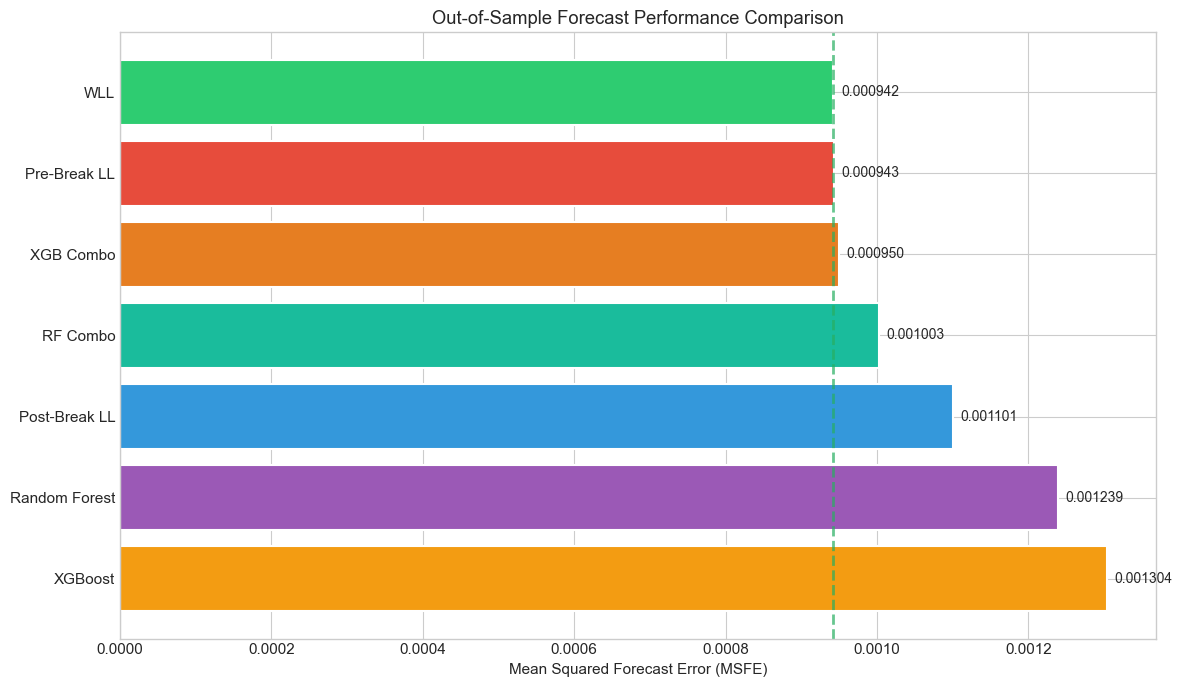
\includegraphics[keepaspectratio]{WLL_Cocoa_Experiment final_files/figure-pdf/cell-19-output-1.png}}

\begin{Shaded}
\begin{Highlighting}[]
\CommentTok{\# Cumulative squared error over time}
\NormalTok{fig, ax }\OperatorTok{=}\NormalTok{ plt.subplots(figsize}\OperatorTok{=}\NormalTok{(}\DecValTok{14}\NormalTok{, }\DecValTok{7}\NormalTok{))}

\ControlFlowTok{for}\NormalTok{ name, preds }\KeywordTok{in}\NormalTok{ predictions.items():}
\NormalTok{    sq\_err }\OperatorTok{=}\NormalTok{ (y\_test.values }\OperatorTok{{-}}\NormalTok{ preds) }\OperatorTok{**} \DecValTok{2}
\NormalTok{    cum\_se }\OperatorTok{=}\NormalTok{ np.cumsum(sq\_err)}
\NormalTok{    color }\OperatorTok{=}\NormalTok{ model\_colors.get(name, }\StringTok{\textquotesingle{}\#95A5A6\textquotesingle{}}\NormalTok{)}
\NormalTok{    lw }\OperatorTok{=} \DecValTok{3} \ControlFlowTok{if}\NormalTok{ name }\OperatorTok{==} \StringTok{\textquotesingle{}WLL\textquotesingle{}} \ControlFlowTok{else} \FloatTok{1.5}
\NormalTok{    alpha }\OperatorTok{=} \FloatTok{1.0} \ControlFlowTok{if}\NormalTok{ name }\OperatorTok{==} \StringTok{\textquotesingle{}WLL\textquotesingle{}} \ControlFlowTok{else} \FloatTok{0.7}
\NormalTok{    ax.plot(test\_dates, cum\_se, label}\OperatorTok{=}\NormalTok{name, color}\OperatorTok{=}\NormalTok{color, linewidth}\OperatorTok{=}\NormalTok{lw, alpha}\OperatorTok{=}\NormalTok{alpha)}

\NormalTok{ax.set\_xlabel(}\StringTok{\textquotesingle{}Date\textquotesingle{}}\NormalTok{)}
\NormalTok{ax.set\_ylabel(}\StringTok{\textquotesingle{}Cumulative Squared Error\textquotesingle{}}\NormalTok{)}
\NormalTok{ax.set\_title(}\StringTok{\textquotesingle{}Cumulative Out{-}of{-}Sample Squared Forecast Error\textquotesingle{}}\NormalTok{)}
\NormalTok{ax.legend(loc}\OperatorTok{=}\StringTok{\textquotesingle{}upper left\textquotesingle{}}\NormalTok{)}
\NormalTok{ax.grid(}\VariableTok{True}\NormalTok{, alpha}\OperatorTok{=}\FloatTok{0.3}\NormalTok{)}
\NormalTok{plt.tight\_layout()}
\NormalTok{plt.show()}
\end{Highlighting}
\end{Shaded}

\pandocbounded{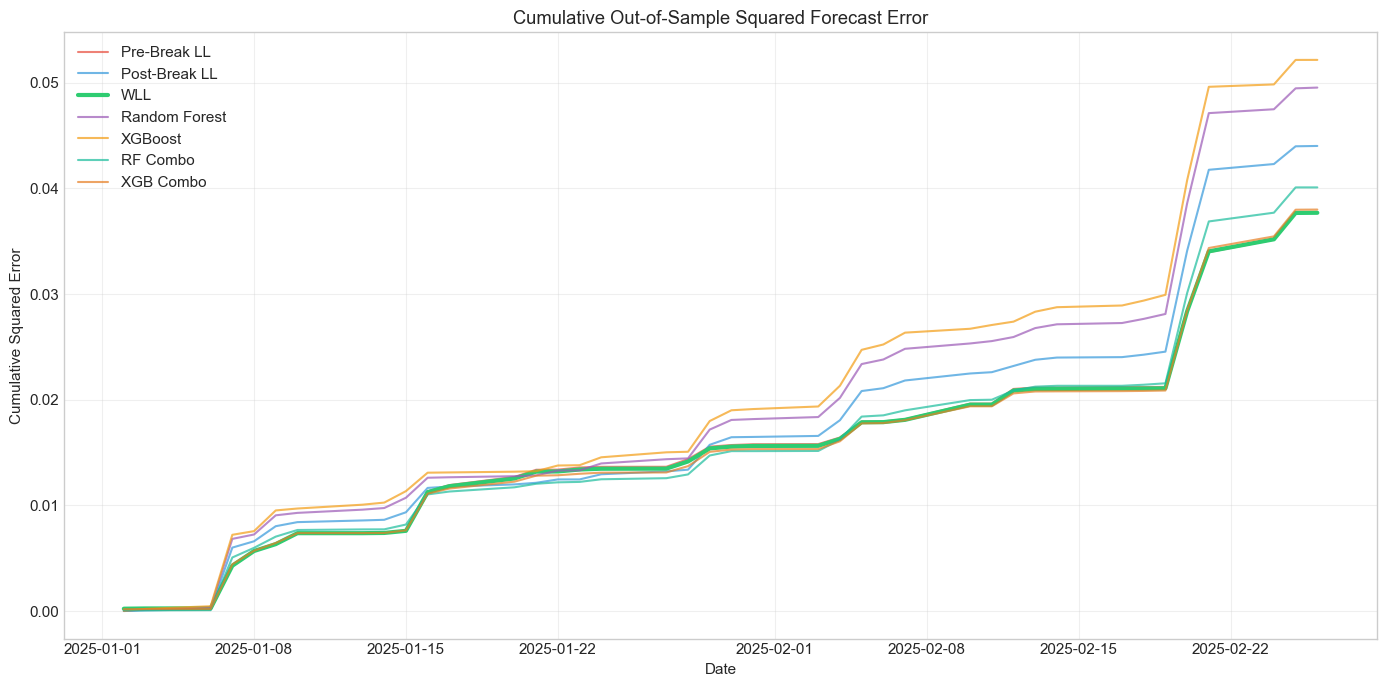
\includegraphics[keepaspectratio]{WLL_Cocoa_Experiment final_files/figure-pdf/cell-20-output-1.png}}

\subsection{7. Modified Diebold-Mariano
Test}\label{modified-diebold-mariano-test}

\begin{Shaded}
\begin{Highlighting}[]
\KeywordTok{def}\NormalTok{ modified\_dm\_test(y\_true, pred1, pred2, h}\OperatorTok{=}\DecValTok{1}\NormalTok{, power}\OperatorTok{=}\DecValTok{2}\NormalTok{):}
    \CommentTok{"""Modified Diebold{-}Mariano test for forecast comparison."""}
\NormalTok{    e1, e2 }\OperatorTok{=}\NormalTok{ y\_true }\OperatorTok{{-}}\NormalTok{ pred1, y\_true }\OperatorTok{{-}}\NormalTok{ pred2}
\NormalTok{    d }\OperatorTok{=}\NormalTok{ np.}\BuiltInTok{abs}\NormalTok{(e1)}\OperatorTok{**}\NormalTok{power }\OperatorTok{{-}}\NormalTok{ np.}\BuiltInTok{abs}\NormalTok{(e2)}\OperatorTok{**}\NormalTok{power}
\NormalTok{    n }\OperatorTok{=} \BuiltInTok{len}\NormalTok{(d)}
\NormalTok{    d\_bar }\OperatorTok{=}\NormalTok{ np.mean(d)}
\NormalTok{    gamma\_0 }\OperatorTok{=}\NormalTok{ np.var(d, ddof}\OperatorTok{=}\DecValTok{1}\NormalTok{)}
    
\NormalTok{    gamma\_sum }\OperatorTok{=} \BuiltInTok{sum}\NormalTok{(}\DecValTok{2} \OperatorTok{*}\NormalTok{ (}\DecValTok{1} \OperatorTok{{-}}\NormalTok{ k}\OperatorTok{/}\NormalTok{h) }\OperatorTok{*}\NormalTok{ np.mean((d[k:] }\OperatorTok{{-}}\NormalTok{ d\_bar) }\OperatorTok{*}\NormalTok{ (d[:}\OperatorTok{{-}}\NormalTok{k] }\OperatorTok{{-}}\NormalTok{ d\_bar))}
                    \ControlFlowTok{for}\NormalTok{ k }\KeywordTok{in} \BuiltInTok{range}\NormalTok{(}\DecValTok{1}\NormalTok{, h))}
\NormalTok{    var\_d }\OperatorTok{=}\NormalTok{ (gamma\_0 }\OperatorTok{+}\NormalTok{ gamma\_sum) }\OperatorTok{/}\NormalTok{ n}
    
    \ControlFlowTok{if}\NormalTok{ var\_d }\OperatorTok{\textless{}=} \DecValTok{0}\NormalTok{:}
        \ControlFlowTok{return}\NormalTok{ np.nan, np.nan}
    
\NormalTok{    dm\_stat }\OperatorTok{=}\NormalTok{ d\_bar }\OperatorTok{/}\NormalTok{ np.sqrt(var\_d)}
\NormalTok{    correction }\OperatorTok{=}\NormalTok{ np.sqrt((n }\OperatorTok{+} \DecValTok{1} \OperatorTok{{-}} \DecValTok{2}\OperatorTok{*}\NormalTok{h }\OperatorTok{+}\NormalTok{ h}\OperatorTok{*}\NormalTok{(h}\OperatorTok{{-}}\DecValTok{1}\NormalTok{)}\OperatorTok{/}\NormalTok{n) }\OperatorTok{/}\NormalTok{ n)}
\NormalTok{    mdm\_stat }\OperatorTok{=}\NormalTok{ dm\_stat }\OperatorTok{*}\NormalTok{ correction}
\NormalTok{    p\_value }\OperatorTok{=} \DecValTok{2} \OperatorTok{*}\NormalTok{ stats.t.sf(np.}\BuiltInTok{abs}\NormalTok{(mdm\_stat), df}\OperatorTok{=}\NormalTok{n}\OperatorTok{{-}}\DecValTok{1}\NormalTok{)}
    \ControlFlowTok{return}\NormalTok{ mdm\_stat, p\_value}

\CommentTok{\# Pairwise MDM tests}
\NormalTok{y\_true\_arr }\OperatorTok{=}\NormalTok{ y\_test.values}
\NormalTok{model\_names }\OperatorTok{=} \BuiltInTok{list}\NormalTok{(predictions.keys())}

\NormalTok{mdm\_matrix }\OperatorTok{=}\NormalTok{ pd.DataFrame(index}\OperatorTok{=}\NormalTok{model\_names, columns}\OperatorTok{=}\NormalTok{model\_names, dtype}\OperatorTok{=}\BuiltInTok{float}\NormalTok{)}
\NormalTok{pval\_matrix }\OperatorTok{=}\NormalTok{ pd.DataFrame(index}\OperatorTok{=}\NormalTok{model\_names, columns}\OperatorTok{=}\NormalTok{model\_names, dtype}\OperatorTok{=}\BuiltInTok{float}\NormalTok{)}

\ControlFlowTok{for}\NormalTok{ m1 }\KeywordTok{in}\NormalTok{ model\_names:}
    \ControlFlowTok{for}\NormalTok{ m2 }\KeywordTok{in}\NormalTok{ model\_names:}
        \ControlFlowTok{if}\NormalTok{ m1 }\OperatorTok{==}\NormalTok{ m2:}
\NormalTok{            mdm\_matrix.loc[m1, m2] }\OperatorTok{=} \FloatTok{0.0}
\NormalTok{            pval\_matrix.loc[m1, m2] }\OperatorTok{=} \FloatTok{1.0}
        \ControlFlowTok{else}\NormalTok{:}
\NormalTok{            stat, pval }\OperatorTok{=}\NormalTok{ modified\_dm\_test(y\_true\_arr, predictions[m1], predictions[m2])}
\NormalTok{            mdm\_matrix.loc[m1, m2] }\OperatorTok{=}\NormalTok{ stat}
\NormalTok{            pval\_matrix.loc[m1, m2] }\OperatorTok{=}\NormalTok{ pval}

\BuiltInTok{print}\NormalTok{(}\StringTok{\textquotesingle{}MDM Test Statistics (positive = row model worse than column):\textquotesingle{}}\NormalTok{)}
\BuiltInTok{print}\NormalTok{(mdm\_matrix.}\BuiltInTok{round}\NormalTok{(}\DecValTok{3}\NormalTok{).to\_string())}
\BuiltInTok{print}\NormalTok{(}\StringTok{\textquotesingle{}}\CharTok{\textbackslash{}n}\StringTok{P{-}Values:\textquotesingle{}}\NormalTok{)}
\BuiltInTok{print}\NormalTok{(pval\_matrix.}\BuiltInTok{round}\NormalTok{(}\DecValTok{3}\NormalTok{).to\_string())}
\end{Highlighting}
\end{Shaded}

\begin{verbatim}
MDM Test Statistics (positive = row model worse than column):
               Pre-Break LL  Post-Break LL    WLL  Random Forest  XGBoost  RF Combo  XGB Combo
Pre-Break LL          0.000         -1.218  0.062         -1.733   -1.930    -0.807     -0.336
Post-Break LL         1.218          0.000  1.285         -3.218   -3.324     1.715      1.387
WLL                  -0.062         -1.285  0.000         -1.804   -2.000    -0.889     -0.503
Random Forest         1.733          3.218  1.804          0.000   -3.396     2.435      1.932
XGBoost               1.930          3.324  2.000          3.396    0.000     2.659      2.134
RF Combo              0.807         -1.715  0.889         -2.435   -2.659     0.000      0.998
XGB Combo             0.336         -1.387  0.503         -1.932   -2.134    -0.998      0.000

P-Values:
               Pre-Break LL  Post-Break LL    WLL  Random Forest  XGBoost  RF Combo  XGB Combo
Pre-Break LL          1.000          0.231  0.951          0.091    0.061     0.425      0.738
Post-Break LL         0.231          1.000  0.206          0.003    0.002     0.094      0.173
WLL                   0.951          0.206  1.000          0.079    0.052     0.379      0.618
Random Forest         0.091          0.003  0.079          1.000    0.002     0.020      0.061
XGBoost               0.061          0.002  0.052          0.002    1.000     0.011      0.039
RF Combo              0.425          0.094  0.379          0.020    0.011     1.000      0.324
XGB Combo             0.738          0.173  0.618          0.061    0.039     0.324      1.000
\end{verbatim}

\subsection{8. Summary}\label{summary}

\begin{Shaded}
\begin{Highlighting}[]
\BuiltInTok{print}\NormalTok{(}\StringTok{\textquotesingle{}=\textquotesingle{}}\OperatorTok{*}\DecValTok{70}\NormalTok{)}
\BuiltInTok{print}\NormalTok{(}\StringTok{\textquotesingle{}EXPERIMENT SUMMARY\textquotesingle{}}\NormalTok{)}
\BuiltInTok{print}\NormalTok{(}\StringTok{\textquotesingle{}=\textquotesingle{}}\OperatorTok{*}\DecValTok{70}\NormalTok{)}

\BuiltInTok{print}\NormalTok{(}\SpecialStringTok{f\textquotesingle{}}\CharTok{\textbackslash{}n}\SpecialStringTok{Data:\textquotesingle{}}\NormalTok{)}
\BuiltInTok{print}\NormalTok{(}\SpecialStringTok{f\textquotesingle{}  Training: }\SpecialCharTok{\{}\NormalTok{df[}\StringTok{"date"}\NormalTok{]}\SpecialCharTok{.}\BuiltInTok{min}\NormalTok{()}\SpecialCharTok{.}\NormalTok{strftime(}\StringTok{"\%Y{-}\%m{-}}\SpecialCharTok{\%d}\StringTok{"}\NormalTok{)}\SpecialCharTok{\}}\SpecialStringTok{ to }\SpecialCharTok{\{}\NormalTok{OOS\_DATE}\SpecialCharTok{.}\NormalTok{strftime(}\StringTok{"\%Y{-}\%m{-}}\SpecialCharTok{\%d}\StringTok{"}\NormalTok{)}\SpecialCharTok{\}}\SpecialStringTok{\textquotesingle{}}\NormalTok{)}
\BuiltInTok{print}\NormalTok{(}\SpecialStringTok{f\textquotesingle{}  Test: }\SpecialCharTok{\{}\NormalTok{OOS\_DATE}\SpecialCharTok{.}\NormalTok{strftime(}\StringTok{"\%Y{-}\%m{-}}\SpecialCharTok{\%d}\StringTok{"}\NormalTok{)}\SpecialCharTok{\}}\SpecialStringTok{ to }\SpecialCharTok{\{}\NormalTok{df[}\StringTok{"date"}\NormalTok{]}\SpecialCharTok{.}\BuiltInTok{max}\NormalTok{()}\SpecialCharTok{.}\NormalTok{strftime(}\StringTok{"\%Y{-}\%m{-}}\SpecialCharTok{\%d}\StringTok{"}\NormalTok{)}\SpecialCharTok{\}}\SpecialStringTok{\textquotesingle{}}\NormalTok{)}
\BuiltInTok{print}\NormalTok{(}\SpecialStringTok{f\textquotesingle{}  Structural break: }\SpecialCharTok{\{}\NormalTok{BREAK\_DATE}\SpecialCharTok{.}\NormalTok{strftime(}\StringTok{"\%Y{-}\%m{-}}\SpecialCharTok{\%d}\StringTok{"}\NormalTok{)}\SpecialCharTok{\}}\SpecialStringTok{\textquotesingle{}}\NormalTok{)}

\BuiltInTok{print}\NormalTok{(}\SpecialStringTok{f\textquotesingle{}}\CharTok{\textbackslash{}n}\SpecialStringTok{Hyperparameters:\textquotesingle{}}\NormalTok{)}
\BuiltInTok{print}\NormalTok{(}\SpecialStringTok{f\textquotesingle{}  Pre{-}break bandwidth: }\SpecialCharTok{\{}\NormalTok{bw\_pre}\SpecialCharTok{:.6f\}}\SpecialStringTok{\textquotesingle{}}\NormalTok{)}
\BuiltInTok{print}\NormalTok{(}\SpecialStringTok{f\textquotesingle{}  Post{-}break bandwidth: }\SpecialCharTok{\{}\NormalTok{bw\_post}\SpecialCharTok{:.6f\}}\SpecialStringTok{\textquotesingle{}}\NormalTok{)}
\BuiltInTok{print}\NormalTok{(}\SpecialStringTok{f\textquotesingle{}  WLL gamma: }\SpecialCharTok{\{}\NormalTok{best\_gamma}\SpecialCharTok{:.4f\}}\SpecialStringTok{\textquotesingle{}}\NormalTok{)}
\BuiltInTok{print}\NormalTok{(}\SpecialStringTok{f\textquotesingle{}  RF Combo gamma: }\SpecialCharTok{\{}\NormalTok{best\_gamma\_rf}\SpecialCharTok{:.4f\}}\SpecialStringTok{\textquotesingle{}}\NormalTok{)}
\BuiltInTok{print}\NormalTok{(}\SpecialStringTok{f\textquotesingle{}  XGB Combo gamma: }\SpecialCharTok{\{}\NormalTok{best\_gamma\_xgb}\SpecialCharTok{:.4f\}}\SpecialStringTok{\textquotesingle{}}\NormalTok{)}

\BuiltInTok{print}\NormalTok{(}\SpecialStringTok{f\textquotesingle{}}\CharTok{\textbackslash{}n}\SpecialStringTok{Results (MSFE):\textquotesingle{}}\NormalTok{)}
\ControlFlowTok{for}\NormalTok{ \_, row }\KeywordTok{in}\NormalTok{ results\_df.iterrows():}
    \BuiltInTok{print}\NormalTok{(}\SpecialStringTok{f\textquotesingle{}  }\SpecialCharTok{\{}\NormalTok{row[}\StringTok{"Rank"}\NormalTok{]}\SpecialCharTok{\}}\SpecialStringTok{. }\SpecialCharTok{\{}\NormalTok{row[}\StringTok{"Model"}\NormalTok{]}\SpecialCharTok{\}}\SpecialStringTok{: }\SpecialCharTok{\{}\NormalTok{row[}\StringTok{"MSFE"}\NormalTok{]}\SpecialCharTok{:.8f\}}\SpecialStringTok{ (}\SpecialCharTok{\{}\NormalTok{row[}\StringTok{"Relative (\%)"}\NormalTok{]}\SpecialCharTok{:.2f\}}\SpecialStringTok{\%)\textquotesingle{}}\NormalTok{)}

\NormalTok{wll\_msfe }\OperatorTok{=}\NormalTok{ results[}\StringTok{\textquotesingle{}WLL\textquotesingle{}}\NormalTok{]}
\NormalTok{post\_msfe }\OperatorTok{=}\NormalTok{ results[}\StringTok{\textquotesingle{}Post{-}Break LL\textquotesingle{}}\NormalTok{]}
\NormalTok{best\_ml }\OperatorTok{=} \BuiltInTok{min}\NormalTok{([}\StringTok{\textquotesingle{}Random Forest\textquotesingle{}}\NormalTok{, }\StringTok{\textquotesingle{}XGBoost\textquotesingle{}}\NormalTok{], key}\OperatorTok{=}\KeywordTok{lambda}\NormalTok{ x: results[x])}
\NormalTok{best\_ml\_msfe }\OperatorTok{=}\NormalTok{ results[best\_ml]}

\BuiltInTok{print}\NormalTok{(}\SpecialStringTok{f\textquotesingle{}}\CharTok{\textbackslash{}n}\SpecialStringTok{Key Comparisons:\textquotesingle{}}\NormalTok{)}
\BuiltInTok{print}\NormalTok{(}\SpecialStringTok{f\textquotesingle{}  WLL vs Post{-}Break LL: }\SpecialCharTok{\{}\NormalTok{(wll\_msfe}\OperatorTok{/}\NormalTok{post\_msfe }\OperatorTok{{-}} \DecValTok{1}\NormalTok{)}\OperatorTok{*}\DecValTok{100}\SpecialCharTok{:+.2f\}}\SpecialStringTok{\%\textquotesingle{}}\NormalTok{)}
\BuiltInTok{print}\NormalTok{(}\SpecialStringTok{f\textquotesingle{}  WLL vs }\SpecialCharTok{\{}\NormalTok{best\_ml}\SpecialCharTok{\}}\SpecialStringTok{: }\SpecialCharTok{\{}\NormalTok{(wll\_msfe}\OperatorTok{/}\NormalTok{best\_ml\_msfe }\OperatorTok{{-}} \DecValTok{1}\NormalTok{)}\OperatorTok{*}\DecValTok{100}\SpecialCharTok{:+.2f\}}\SpecialStringTok{\%\textquotesingle{}}\NormalTok{)}

\BuiltInTok{print}\NormalTok{(}\StringTok{\textquotesingle{}}\CharTok{\textbackslash{}n}\StringTok{\textquotesingle{}} \OperatorTok{+} \StringTok{\textquotesingle{}=\textquotesingle{}}\OperatorTok{*}\DecValTok{70}\NormalTok{)}
\end{Highlighting}
\end{Shaded}

\begin{verbatim}
======================================================================
EXPERIMENT SUMMARY
======================================================================

Data:
  Training: 1994-10-04 to 2025-01-02
  Test: 2025-01-02 to 2025-02-26
  Structural break: 2022-09-23

Hyperparameters:
  Pre-break bandwidth: 1.717366
  Post-break bandwidth: 1.717366
  WLL gamma: 0.9500
  RF Combo gamma: 0.7000
  XGB Combo gamma: 1.0000

Results (MSFE):
  1. WLL: 0.00094248 (0.00%)
  2. Pre-Break LL: 0.00094288 (0.04%)
  3. XGB Combo: 0.00095010 (0.81%)
  4. RF Combo: 0.00100254 (6.37%)
  5. Post-Break LL: 0.00110062 (16.78%)
  6. Random Forest: 0.00123874 (31.43%)
  7. XGBoost: 0.00130428 (38.39%)

Key Comparisons:
  WLL vs Post-Break LL: -14.37%
  WLL vs Random Forest: -23.92%

======================================================================
\end{verbatim}

\begin{Shaded}
\begin{Highlighting}[]
\CommentTok{\# Save results}
\NormalTok{output\_dir }\OperatorTok{=}\NormalTok{ Path.cwd().parent }\OperatorTok{/} \StringTok{\textquotesingle{}output\textquotesingle{}} \OperatorTok{/} \StringTok{\textquotesingle{}experiment\_results\textquotesingle{}}
\NormalTok{output\_dir.mkdir(parents}\OperatorTok{=}\VariableTok{True}\NormalTok{, exist\_ok}\OperatorTok{=}\VariableTok{True}\NormalTok{)}

\NormalTok{timestamp }\OperatorTok{=}\NormalTok{ datetime.now().strftime(}\StringTok{\textquotesingle{}\%Y\%m}\SpecialCharTok{\%d}\StringTok{\_\%H\%M\%S\textquotesingle{}}\NormalTok{)}

\NormalTok{results\_df.to\_csv(output\_dir }\OperatorTok{/} \SpecialStringTok{f\textquotesingle{}msfe\_results\_}\SpecialCharTok{\{}\NormalTok{timestamp}\SpecialCharTok{\}}\SpecialStringTok{.csv\textquotesingle{}}\NormalTok{, index}\OperatorTok{=}\VariableTok{False}\NormalTok{)}
\NormalTok{mdm\_matrix.to\_csv(output\_dir }\OperatorTok{/} \SpecialStringTok{f\textquotesingle{}mdm\_statistics\_}\SpecialCharTok{\{}\NormalTok{timestamp}\SpecialCharTok{\}}\SpecialStringTok{.csv\textquotesingle{}}\NormalTok{)}
\NormalTok{pval\_matrix.to\_csv(output\_dir }\OperatorTok{/} \SpecialStringTok{f\textquotesingle{}mdm\_pvalues\_}\SpecialCharTok{\{}\NormalTok{timestamp}\SpecialCharTok{\}}\SpecialStringTok{.csv\textquotesingle{}}\NormalTok{)}

\NormalTok{pred\_df }\OperatorTok{=}\NormalTok{ pd.DataFrame(predictions)}
\NormalTok{pred\_df[}\StringTok{\textquotesingle{}date\textquotesingle{}}\NormalTok{] }\OperatorTok{=}\NormalTok{ test\_dates.values}
\NormalTok{pred\_df[}\StringTok{\textquotesingle{}y\_true\textquotesingle{}}\NormalTok{] }\OperatorTok{=}\NormalTok{ y\_test.values}
\NormalTok{pred\_df.to\_csv(output\_dir }\OperatorTok{/} \SpecialStringTok{f\textquotesingle{}predictions\_}\SpecialCharTok{\{}\NormalTok{timestamp}\SpecialCharTok{\}}\SpecialStringTok{.csv\textquotesingle{}}\NormalTok{, index}\OperatorTok{=}\VariableTok{False}\NormalTok{)}

\BuiltInTok{print}\NormalTok{(}\SpecialStringTok{f\textquotesingle{}Results saved to: }\SpecialCharTok{\{}\NormalTok{output\_dir}\SpecialCharTok{\}}\SpecialStringTok{\textquotesingle{}}\NormalTok{)}
\end{Highlighting}
\end{Shaded}

\begin{verbatim}
Results saved to: w:\Research\NP\Cocoa\output\experiment_results
\end{verbatim}

\#\# Hypotheses and how we test them

Main question: does explicit break-aware weighting (WLL) adapt faster
and give better post-break forecasts than break-agnostic ML (RF, XGB)?

\begin{itemize}
\tightlist
\item
  H0 (overall): On the post-break test sample, WLL MSFE \textless{} RF
  and WLL MSFE \textless{} XGB.
\item
  H1 (early): In the first K days of the post-break test, the WLL
  cumulative squared error grows slower than RF and XGB.
\end{itemize}

Data/timeline note: break detected at 2022-09-23; current OOS test
starts 2025-01- 02 with 40 points. ``Early'' here means the first K test
days. To make the adaptation

How we check: - Use the saved \texttt{predictions\_*.csv} from the main
run. - Compute overall MSFE for WLL, RF, XGB (H0). - Compute and exame
MSFE on short windows (1--20, 21--40) and the winning model in each
state

\begin{Shaded}
\begin{Highlighting}[]
\ImportTok{from}\NormalTok{ pathlib }\ImportTok{import}\NormalTok{ Path}
\ImportTok{import}\NormalTok{ pandas }\ImportTok{as}\NormalTok{ pd}
\ImportTok{import}\NormalTok{ numpy }\ImportTok{as}\NormalTok{ np}

\CommentTok{\# Load latest predictions file}
\NormalTok{pred\_dir }\OperatorTok{=}\NormalTok{ Path.cwd().parent }\OperatorTok{/} \StringTok{"output"} \OperatorTok{/} \StringTok{"experiment\_results"}
\NormalTok{pred\_file }\OperatorTok{=} \BuiltInTok{sorted}\NormalTok{(pred\_dir.glob(}\StringTok{"predictions\_*.csv"}\NormalTok{))[}\OperatorTok{{-}}\DecValTok{1}\NormalTok{]}
\NormalTok{pred\_use }\OperatorTok{=}\NormalTok{ pd.read\_csv(pred\_file).sort\_values(}\StringTok{\textquotesingle{}date\textquotesingle{}}\NormalTok{).reset\_index(drop}\OperatorTok{=}\VariableTok{True}\NormalTok{)}

\NormalTok{models\_to\_check }\OperatorTok{=}\NormalTok{ [}\StringTok{"WLL"}\NormalTok{, }\StringTok{"Random Forest"}\NormalTok{, }\StringTok{"XGBoost"}\NormalTok{]}
\NormalTok{y\_true }\OperatorTok{=}\NormalTok{ pred\_use[}\StringTok{"y\_true"}\NormalTok{].to\_numpy()}
\NormalTok{dates }\OperatorTok{=}\NormalTok{ pd.to\_datetime(pred\_use[}\StringTok{"date"}\NormalTok{])}

\BuiltInTok{print}\NormalTok{(}\SpecialStringTok{f"Loaded predictions file: }\SpecialCharTok{\{}\NormalTok{pred\_file}\SpecialCharTok{.}\NormalTok{name}\SpecialCharTok{\}}\SpecialStringTok{"}\NormalTok{)}
\end{Highlighting}
\end{Shaded}

\begin{verbatim}
Loaded predictions file: predictions_20251201_205941.csv
\end{verbatim}

\begin{Shaded}
\begin{Highlighting}[]
\CommentTok{\# H1: overall post{-}break MSFE}

\ImportTok{import}\NormalTok{ numpy }\ImportTok{as}\NormalTok{ np}

\KeywordTok{def}\NormalTok{ msfe(y, yhat):}
    \ControlFlowTok{return}\NormalTok{ np.mean((y }\OperatorTok{{-}}\NormalTok{ yhat) }\OperatorTok{**} \DecValTok{2}\NormalTok{)}

\NormalTok{msfe\_rows }\OperatorTok{=}\NormalTok{ []}
\ControlFlowTok{for}\NormalTok{ m }\KeywordTok{in}\NormalTok{ models\_to\_check:}
\NormalTok{    m\_msfe }\OperatorTok{=}\NormalTok{ msfe(y\_true, pred\_use[m].to\_numpy())}
\NormalTok{    msfe\_rows.append(\{}\StringTok{"Model"}\NormalTok{: m, }\StringTok{"MSFE"}\NormalTok{: m\_msfe\})}

\NormalTok{msfe\_df }\OperatorTok{=}\NormalTok{ pd.DataFrame(msfe\_rows)}
\NormalTok{wll\_msfe }\OperatorTok{=}\NormalTok{ msfe\_df.loc[msfe\_df[}\StringTok{"Model"}\NormalTok{] }\OperatorTok{==} \StringTok{"WLL"}\NormalTok{, }\StringTok{"MSFE"}\NormalTok{].values[}\DecValTok{0}\NormalTok{]}
\NormalTok{msfe\_df[}\StringTok{"Rel\_to\_WLL\_\%"}\NormalTok{] }\OperatorTok{=}\NormalTok{ (msfe\_df[}\StringTok{"MSFE"}\NormalTok{] }\OperatorTok{/}\NormalTok{ wll\_msfe }\OperatorTok{{-}} \DecValTok{1}\NormalTok{) }\OperatorTok{*} \DecValTok{100}
\NormalTok{msfe\_df.sort\_values(}\StringTok{"MSFE"}\NormalTok{)}
\end{Highlighting}
\end{Shaded}

\begin{longtable}[]{@{}llll@{}}
\toprule\noalign{}
& Model & MSFE & Rel\_to\_WLL\_\% \\
\midrule\noalign{}
\endhead
\bottomrule\noalign{}
\endlastfoot
0 & WLL & 0.000942 & 0.000000 \\
1 & Random Forest & 0.001239 & 31.433508 \\
2 & XGBoost & 0.001304 & 38.387814 \\
\end{longtable}

\begin{Shaded}
\begin{Highlighting}[]
\CommentTok{\# H2: early post{-}break cumulative squared error}
\NormalTok{early\_k }\OperatorTok{=} \DecValTok{60}  \CommentTok{\# adjust window length as needed}
\NormalTok{early\_df }\OperatorTok{=}\NormalTok{ pred\_use.iloc[:early\_k].copy()}

\NormalTok{cse\_df }\OperatorTok{=}\NormalTok{ pd.DataFrame(\{}\StringTok{"date"}\NormalTok{: pd.to\_datetime(early\_df[}\StringTok{"date"}\NormalTok{] )\})}
\ControlFlowTok{for}\NormalTok{ m }\KeywordTok{in}\NormalTok{ models\_to\_check:}
\NormalTok{    se }\OperatorTok{=}\NormalTok{ (early\_df[}\StringTok{"y\_true"}\NormalTok{] }\OperatorTok{{-}}\NormalTok{ early\_df[m]) }\OperatorTok{**} \DecValTok{2}
\NormalTok{    cse\_df[}\SpecialStringTok{f"CSE\_}\SpecialCharTok{\{}\NormalTok{m}\SpecialCharTok{\}}\SpecialStringTok{"}\NormalTok{] }\OperatorTok{=}\NormalTok{ se.cumsum()}

\NormalTok{cse\_df.head()}
\end{Highlighting}
\end{Shaded}

\begin{longtable}[]{@{}lllll@{}}
\toprule\noalign{}
& date & CSE\_WLL & CSE\_Random Forest & CSE\_XGBoost \\
\midrule\noalign{}
\endhead
\bottomrule\noalign{}
\endlastfoot
0 & 2025-01-02 & 0.000223 & 0.000004 & 0.000014 \\
1 & 2025-01-03 & 0.000246 & 0.000152 & 0.000207 \\
2 & 2025-01-06 & 0.000254 & 0.000353 & 0.000459 \\
3 & 2025-01-07 & 0.004293 & 0.006832 & 0.007218 \\
4 & 2025-01-08 & 0.005685 & 0.007247 & 0.007566 \\
\end{longtable}

\begin{Shaded}
\begin{Highlighting}[]
\ImportTok{import}\NormalTok{ matplotlib.pyplot }\ImportTok{as}\NormalTok{ plt}

\NormalTok{plt.figure(figsize}\OperatorTok{=}\NormalTok{(}\DecValTok{10}\NormalTok{, }\DecValTok{5}\NormalTok{))}
\ControlFlowTok{for}\NormalTok{ m }\KeywordTok{in}\NormalTok{ models\_to\_check:}
\NormalTok{    plt.plot(cse\_df[}\StringTok{"date"}\NormalTok{], cse\_df[}\SpecialStringTok{f"CSE\_}\SpecialCharTok{\{}\NormalTok{m}\SpecialCharTok{\}}\SpecialStringTok{"}\NormalTok{], label}\OperatorTok{=}\NormalTok{m)}

\NormalTok{plt.xlabel(}\StringTok{"Date"}\NormalTok{)}
\NormalTok{plt.ylabel(}\StringTok{"Cumulative squared error"}\NormalTok{)}
\NormalTok{plt.title(}\SpecialStringTok{f"Early post{-}break CSE (first }\SpecialCharTok{\{}\NormalTok{early\_k}\SpecialCharTok{\}}\SpecialStringTok{ observations)"}\NormalTok{)}
\NormalTok{plt.legend()}
\NormalTok{plt.grid(}\VariableTok{True}\NormalTok{, linestyle}\OperatorTok{=}\StringTok{"{-}{-}"}\NormalTok{, alpha}\OperatorTok{=}\FloatTok{0.5}\NormalTok{)}
\NormalTok{plt.show()}
\end{Highlighting}
\end{Shaded}

\pandocbounded{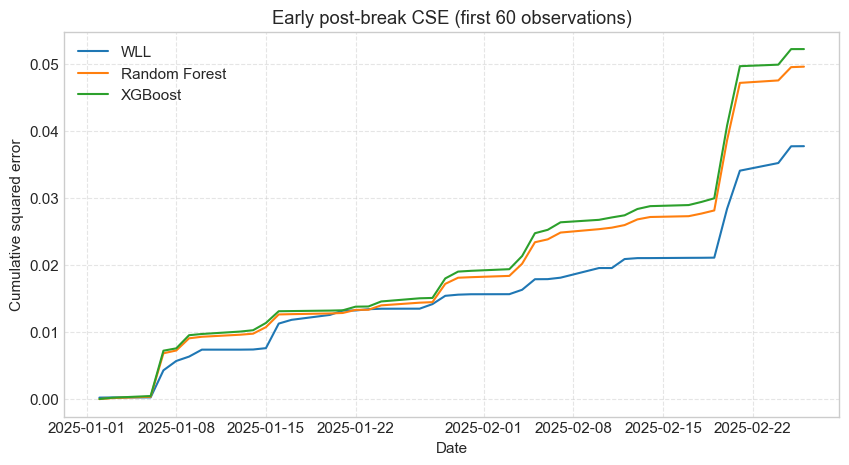
\includegraphics[keepaspectratio]{WLL_Cocoa_Experiment final_files/figure-pdf/cell-27-output-1.png}}

\begin{Shaded}
\begin{Highlighting}[]
\CommentTok{\# Scalar summary at day K}
\NormalTok{cse\_end }\OperatorTok{=}\NormalTok{ \{m: cse\_df[}\SpecialStringTok{f"CSE\_}\SpecialCharTok{\{}\NormalTok{m}\SpecialCharTok{\}}\SpecialStringTok{"}\NormalTok{].iloc[}\OperatorTok{{-}}\DecValTok{1}\NormalTok{] }\ControlFlowTok{for}\NormalTok{ m }\KeywordTok{in}\NormalTok{ models\_to\_check\}}

\NormalTok{cse\_summary }\OperatorTok{=}\NormalTok{ (}
\NormalTok{    pd.DataFrame(\{}
        \StringTok{"Model"}\NormalTok{: models\_to\_check,}
        \StringTok{"CSE\_first\_K"}\NormalTok{: [cse\_end[m] }\ControlFlowTok{for}\NormalTok{ m }\KeywordTok{in}\NormalTok{ models\_to\_check],}
\NormalTok{    \})}
\NormalTok{    .assign(}\OperatorTok{**}\NormalTok{\{}\StringTok{\textquotesingle{}Rel\_to\_WLL\_\%\textquotesingle{}}\NormalTok{: }\KeywordTok{lambda}\NormalTok{ df: (df[}\StringTok{\textquotesingle{}CSE\_first\_K\textquotesingle{}}\NormalTok{] }\OperatorTok{/}\NormalTok{ df.loc[df[}\StringTok{\textquotesingle{}Model\textquotesingle{}}\NormalTok{] }\OperatorTok{==} \StringTok{\textquotesingle{}WLL\textquotesingle{}}\NormalTok{, }\StringTok{\textquotesingle{}CSE\_first\_K\textquotesingle{}}\NormalTok{].values[}\DecValTok{0}\NormalTok{] }\OperatorTok{{-}} \DecValTok{1}\NormalTok{) }\OperatorTok{*} \DecValTok{100}\NormalTok{\})}
\NormalTok{)}
\NormalTok{cse\_summary.sort\_values(}\StringTok{"CSE\_first\_K"}\NormalTok{)}
\end{Highlighting}
\end{Shaded}

\begin{longtable}[]{@{}llll@{}}
\toprule\noalign{}
& Model & CSE\_first\_K & Rel\_to\_WLL\_\% \\
\midrule\noalign{}
\endhead
\bottomrule\noalign{}
\endlastfoot
0 & WLL & 0.037699 & 0.000000 \\
1 & Random Forest & 0.049550 & 31.433508 \\
2 & XGBoost & 0.052171 & 38.387814 \\
\end{longtable}

\begin{Shaded}
\begin{Highlighting}[]
\CommentTok{\# Optional: windowed MSFE slices (e.g., 1{-}20, 21{-}40, 41{-}60)}
\NormalTok{n }\OperatorTok{=} \DecValTok{20}  \CommentTok{\# window length (adjust as needed)}
\NormalTok{num\_obs }\OperatorTok{=} \BuiltInTok{len}\NormalTok{(y\_true)}
\NormalTok{windows }\OperatorTok{=}\NormalTok{ [(start, }\BuiltInTok{min}\NormalTok{(start }\OperatorTok{+}\NormalTok{ n, num\_obs)) }\ControlFlowTok{for}\NormalTok{ start }\KeywordTok{in} \BuiltInTok{range}\NormalTok{(}\DecValTok{0}\NormalTok{, num\_obs, n)]}

\NormalTok{win\_rows }\OperatorTok{=}\NormalTok{ []}
\ControlFlowTok{for}\NormalTok{ start, end }\KeywordTok{in}\NormalTok{ windows:}
\NormalTok{    y\_slice }\OperatorTok{=}\NormalTok{ y\_true[start:end]}
    \ControlFlowTok{for}\NormalTok{ m }\KeywordTok{in}\NormalTok{ models\_to\_check:}
\NormalTok{        yhat\_slice }\OperatorTok{=}\NormalTok{ pred\_use[m].to\_numpy()[start:end]}
\NormalTok{        win\_rows.append(\{}
            \StringTok{"Window"}\NormalTok{: }\SpecialStringTok{f"}\SpecialCharTok{\{}\NormalTok{start }\OperatorTok{+} \DecValTok{1}\SpecialCharTok{\}}\SpecialStringTok{{-}}\SpecialCharTok{\{}\NormalTok{end}\SpecialCharTok{\}}\SpecialStringTok{"}\NormalTok{,}
            \StringTok{"Model"}\NormalTok{: m,}
            \StringTok{"MSFE"}\NormalTok{: msfe(y\_slice, yhat\_slice),}
\NormalTok{        \})}

\NormalTok{win\_df }\OperatorTok{=}\NormalTok{ pd.DataFrame(win\_rows)}

\NormalTok{win\_rel }\OperatorTok{=}\NormalTok{ []}
\ControlFlowTok{for}\NormalTok{ window }\KeywordTok{in}\NormalTok{ win\_df[}\StringTok{"Window"}\NormalTok{].unique():}
\NormalTok{    tmp }\OperatorTok{=}\NormalTok{ win\_df[win\_df[}\StringTok{"Window"}\NormalTok{] }\OperatorTok{==}\NormalTok{ window].copy()}
\NormalTok{    wll\_val }\OperatorTok{=}\NormalTok{ tmp.loc[tmp[}\StringTok{"Model"}\NormalTok{] }\OperatorTok{==} \StringTok{"WLL"}\NormalTok{, }\StringTok{"MSFE"}\NormalTok{].values[}\DecValTok{0}\NormalTok{]}
\NormalTok{    tmp[}\StringTok{"Rel\_to\_WLL\_\%"}\NormalTok{] }\OperatorTok{=}\NormalTok{ (tmp[}\StringTok{"MSFE"}\NormalTok{] }\OperatorTok{/}\NormalTok{ wll\_val }\OperatorTok{{-}} \DecValTok{1}\NormalTok{) }\OperatorTok{*} \DecValTok{100}
\NormalTok{    win\_rel.append(tmp)}

\NormalTok{win\_df\_rel }\OperatorTok{=}\NormalTok{ pd.concat(win\_rel, ignore\_index}\OperatorTok{=}\VariableTok{True}\NormalTok{)}
\NormalTok{win\_df\_rel}
\end{Highlighting}
\end{Shaded}

\begin{longtable}[]{@{}lllll@{}}
\toprule\noalign{}
& Window & Model & MSFE & Rel\_to\_WLL\_\% \\
\midrule\noalign{}
\endhead
\bottomrule\noalign{}
\endlastfoot
0 & 1-20 & WLL & 0.000770 & 0.000000 \\
1 & 1-20 & Random Forest & 0.000859 & 11.587360 \\
2 & 1-20 & XGBoost & 0.000899 & 16.836735 \\
3 & 21-40 & WLL & 0.001115 & 0.000000 \\
4 & 21-40 & Random Forest & 0.001619 & 45.131825 \\
5 & 21-40 & XGBoost & 0.001709 & 53.262919 \\
\end{longtable}

Conclusion 1--20 and 45--53\% worse in 21--40). The early CSE curve
stays below both ML curves. so its error grows slower (first-order
``velocity''), not just lower total distance. That is a cleaner
adaptation signal than the final CSE level alone.

DM p-values are weak because the test set is short, but point estimates
favor WLL. Gamma: WLL \textasciitilde0.95; RF Combo 0.7; XGB Combo 1.0.
For a stronger ``fast adaptation'' the previous conclusion




\end{document}
